\documentclass[11pt]{book}
%-------------------PAQUETES-------------------------------
\usepackage{graphicx}
\usepackage[spanish]{babel}
\usepackage{verbatim}
\usepackage{listings}
\usepackage{color}
\usepackage[cache=false]{minted}
\usemintedstyle{coloso}
\usepackage{longtable} 
\usepackage[utf8]{inputenc}
\usepackage{array}
\usepackage{hyperref}
%---------------COMANDOS--------------------
\newcommand{\imagen}[3]{
\begin{figure}[h!]
	\centering
	\includegraphics[width=#1\linewidth]{#2}
	\caption{#3}
\end{figure}
}
%-------------------------------------------
\definecolor{miverde}{rgb}{0,0.6,0}
\definecolor{migris}{rgb}{0.5,0.5,0.5}
\definecolor{mimalva}{rgb}{0.58,0,0.82}

\lstset{ %
	backgroundcolor=\color{white},   % Indica el color de fondo; necesita que se añada \usepackage{color} o \usepackage{xcolor}
	basicstyle=\footnotesize,        % Fija el tamaño del tipo de letra utilizado para el código
	breakatwhitespace=false,         % Activarlo para que los saltos automáticos solo se apliquen en los espacios en blanco
	breaklines=true,                 % Activa el salto de línea automático
	captionpos=b,                    % Establece la posición de la leyenda del cuadro de código
	commentstyle=\color{miverde},    % Estilo de los comentarios
	deletekeywords={...},            % Si se quiere eliminar palabras clave del lenguaje
	escapeinside={\%*}{*)},          % Si quieres incorporar LaTeX dentro del propio código
	extendedchars=true,              % Permite utilizar caracteres extendidos no-ASCII; solo funciona para codificaciones de 8-bits; para UTF-8 no funciona. En xelatex necesita estar a true para que funcione.
	frame=single,	                   % Añade un marco al código
	keepspaces=true,                 % Mantiene los espacios en el texto. Es útil para mantener la indentación del código(puede necesitar columns=flexible).
	keywordstyle=\color{blue},       % estilo de las palabras clave
	language=Java,                 % El lenguaje del código
	otherkeywords={*,...},           % Si se quieren añadir otras palabras clave al lenguaje
	numbers=left,                    % Posición de los números de línea (none, left, right).
	numbersep=5pt,                   % Distancia de los números de línea al código
	numberstyle=\small\color{migris}, % Estilo para los números de línea
	rulecolor=\color{black},         % Si no se activa, el color del marco puede cambiar en los saltos de línea entre textos que sea de otro color, por ejemplo, los comentarios, que están en verde en este ejemplo
	showspaces=true,                % Si se activa, muestra los espacios con guiones bajos; sustituye a 'showstringspaces'
	showstringspaces=false,          % subraya solamente los espacios que estén en una cadena de esto
	showtabs=true,                  % muestra las tabulaciones que existan en cadenas de texto con guión bajo
	stepnumber=2,                    % Muestra solamente los números de línea que corresponden a cada salto. En este caso: 1,3,5,...
	stringstyle=\color{mimalva},     % Estilo de las cadenas de texto
	tabsize=2,	                   % Establece el salto de las tabulaciones a 2 espacios
	title=\lstname                   % muestra el nombre de los ficheros incluidos al utilizar \lstinputlisting; también se puede utilizar en el parámetro caption
}
\newmintedfile[CodigoJava]{java}{
	%bgcolor= gray!1!white,
	fontsize=\footnotesize,
	fontfamily=tt,	
	linenos=true,
	numberblanklines=true,
	numbersep=3pt,
	gobble=0,
	%frame=bottomline,
	rulecolor = red!20,
	framerule=0.1pt,
	framesep=0mm,
	funcnamehighlighting=true,
	tabsize=4,
	obeytabs=false,
	mathescape=false
	samepage=false, %with this setting you can force the list to appear on the same page
	showspaces=false,
	showtabs =false,
	texcl=false,
	breaklines=true
}

%----------------------------
\newcommand{\plogo}{\fbox{$\mathcal{PL}$}} % Generic dummy publisher logo

%-------------------MACROS---------------------------------
%-------------------PORTADA--------------------------------
\author{
	Nestor David Bohorquez Galeano \\ 
	20172020083 \\
	Nicolas Herrera Rubiano \\
	20171020118 \\
	Alvaro Andres Niño Rincon \\
	20171020139	
}
\title{Arquitectura Empresarial}

\begin{document}
%\maketitle

\begin{titlepage} % Suppresses headers and footers on the title page
	
	\centering
	\scshape % Use small caps for all text on the title page
	\vspace*{\baselineskip} % White space at the top of the page
	
	\rule{\textwidth}{1.6pt}\vspace*{-\baselineskip}\vspace*{2pt} % Thick horizontal rule
	\rule{\textwidth}{0.4pt} % Thin horizontal rule
	
	\vspace{0.75\baselineskip}
	
	{\LARGE ARQUITECTURA EMPRESARIAL} % Title
	
	\vspace{0.75\baselineskip}
	
	\rule{\textwidth}{0.4pt}\vspace*{-\baselineskip}\vspace{3.2pt} % Thin horizontal rule
	\rule{\textwidth}{1.6pt} % Thick horizontal rule
	
	\vspace{2\baselineskip}
	
	\vspace*{3\baselineskip}
	
	Elaborado Por
	
	\vspace{0.5\baselineskip} 
	
	{\scshape\Large Nestor David Bohorquez Galeano \\ 20172020083 \\ 
	Nicolas Herrera Rubiano \\ 20171020118 \\ 
	Alvaro Andres Niño Rincon \\ 20171020139}
	
	\vspace{0.5\baselineskip} 
	
	\textit{Universidad Distrital Francisco José de Caldas}
	
	\vfill 
	
	\begin{figure}[h!]
		\centering
		
\includegraphics[width=0.3\linewidth]{imgs/ud.jpeg}
	\end{figure}
	
	\today
\end{titlepage}

\tableofcontents
\listoffigures

\part{PROYECTO}
\chapter{Empresa}
\section{Introducción}
En la evolución de la humanidad y las sociedades, la educación ha sido parte fundamental para lograr todo lo que el hombre ha conseguido. La educación ha sido el pilar fundamental sobre el cual se ha construido todos los grandes avances del hombre, toda la tecnología, descubrimientos e infinidad de saberes humanos han sido gracias a la educación, en principio transmitiendo los conocimientos de generación en generación por medio de simples relatos sin ningún tipo de organización y poco a poco este proceso de dar a otros conocimiento ha evolucionado al punto de tener una gran y compleja estructura, bien definida, que busca dar conocimientos por medio de la educación a la sociedad, como se puede evidenciar los colegios, institutos, universidades, etc. De igual manera, se necesita un organismo general que rija la forma de dar educación y que contenidos impartir, porque de lo contrario cada centro educativo enseñaría lo que a su entender le parezca mejor y la sociedad podría recibir diferentes enseñanzas que podrían ser contradictorias. En Colombia, este organismo que rige la educación es el Ministerio de Educación Nacional el cual, a través del tiempo y con el auge de la tecnología ha innovado y se ha adaptado poco a poco a los grandes beneficios que esta conlleva y por tal motivo una estrategia educativa y didáctica para instruir a las futuras generaciones es por medio de un juego, llevando al alumno a entender y comprender que lo compone y no simplemente jugar.

En consecuencia, el Ministerio de Educación Nacional será nuestro objeto de estudio con fines académicos para logar en una primera instancia, comprender su estructura organizacional como paso intermedio para brindar una solución optima a los requerimientos corporativos de la misma, mediante la implementación de los conceptos que iremos desarrollando a lo largo del presente espacio académico.


%\newpage
\section{Organización-Ministerio de Educación \\ Nacional (MEN)}
El Ministerio de Educación Nacional de Colombia es un ministerio de la República de Colombia encargado de formular la política de educación nacional y fomentar el desarrollo de una educación competitiva y de calidad que genere oportunidades de progreso y prosperidad y contribuya a cerrar las brechas de inequidad. Lo anterior, como propósito fundamental sin embargo, a lo largo del tiempo se ha ampliado su visión en busca de transversalidad con diversos campos como la tecnología o el agropecuario con el fin de mejorar cada vez más y más la educación en todos sus aspectos.
Su inicio fue mediante la Ley 10 de 1880 la cual creó la Secretaría de Instrucción Pública, que reemplazó a la Secretaría del Exterior (Ministerio de Gobierno) que antes de 1880 atendía los asuntos educativos.
Mediante la Ley 7 del 25 de agosto de 1886 se creó el Ministerio de Instrucción Pública, durante el gobierno del presidente José María Campo Serrano.
En junio de 1923, cambia el nombre de Ministerio de Instrucción Pública por el de Ministerio de Instrucción y Salubridad Públicas y, desde el 1º de enero de 1928 se le identifica con el nombre de Ministerio de Educación Nacional, según lo dispuso la Ley 56 de 1927 (10 de noviembre), siendo presidente de la República Miguel Abadía Méndez y ministro de Instrucción y Salubridad Públicas José Vicente Huertas. En la actualidad la Ministra de Educación Nacional es María Victoria Angulo desde 2018.

\section{Mision}
Liderar la formulación, implementación y evaluación de políticas públicas educativas, para cerrar las brechas que existen en la garantía del derecho a la educación, y en la prestación de un servicio educativo con calidad, esto en el marco de la atención integral que reconoce e integra la diferencia, los territorios y sus contextos, para permitir trayectorias educativas completas que impulsan el desarrollo integral de los individuos y la sociedad.

\section{Vision}
En 2022, a partir del gran pacto por una educación con enfoque integral desde la primera infancia y a lo largo de la vida, el Ministerio de Educación Nacional habrá liderado con responsabilidad social y financiera, transformaciones estructurales en el sistema educativo de Colombia dirigidas al mejoramiento progresivo de su capacidad para generar condiciones y oportunidades que favorezcan el desarrollo pleno de las personas y sus comunidades, soportado en el fortalecimiento de las capacidades sectoriales y territoriales requeridas para garantizar el cierre de brechas de acceso, permanencia y calidad en el entorno urbano y, especialmente en el rural.


\newpage
\section{Objetivos}

\subsection{General}
El Plan Nacional Decenal de Educación 2016-2026, PNDE 2016-2026 traza la ruta de Colombia en Educación en los próximos 10 años, hacia “un sistema educativo de calidad que promueva el desarrollo económico y social del país, y la construcción de una sociedad cuyos cimientos sean la justicia, el respeto y el reconocimiento de las diferencias”. Este documento surge de un proceso de construcción colectiva, con una amplia participación
municipal, departamental, regional y nacional, de los colombianos de todas las ciudades y etnias.

\subsection{Específicos}
Tomando como referencia el objetivo general, se definieron 10 lineamientos estratégicos que permitirán resolver los desafíos planteados a 2026, los cuales se
mencionan a continuación:

\begin{enumerate}
	\item Regular y precisar el alcance del derecho a la educación.
	\item Construcción de un sistema educativo articulado, participativo,
	descentralizado y con mecanismos eficaces de concertación.
	Plan Estratégico Institucional 2019-2022
	\item Establecimiento de lineamientos curriculares generales, pertinentes y flexibles.
	\item Construcción de una política pública para la formación de educadores.
	\item  Impulsar una educación que transforme el paradigma que ha dominado hasta el momento.
	\item Impulsar el uso pertinente, pedagógico y generalizado de las nuevas diversas tecnologías para apoyar la enseñanza, la construcción de conocimiento, el aprendizaje, la investigación y la innovación, fortaleciendo el desarrollo para la vida.
	\item Construir una red sociedad en paz sobre una base de equidad, inclusión, respeto a la ética y equidad de género.
	\item Dar prioridad al desarrollo de la población rural a partir de la educación.
	\item La importancia otorgada por el estado a la educación se medirá por
	la participación del gasto educativo en el PIB y en el gasto del Gobierno, en todos sus niveles administrativos.
	\item Fomentar la investigación que lleve a la generación de conocimiento en todos los niveles de la educación.
\end{enumerate}


%\newpage
\section{Organigrama}

\begin{figure}[h!]
	\centering
	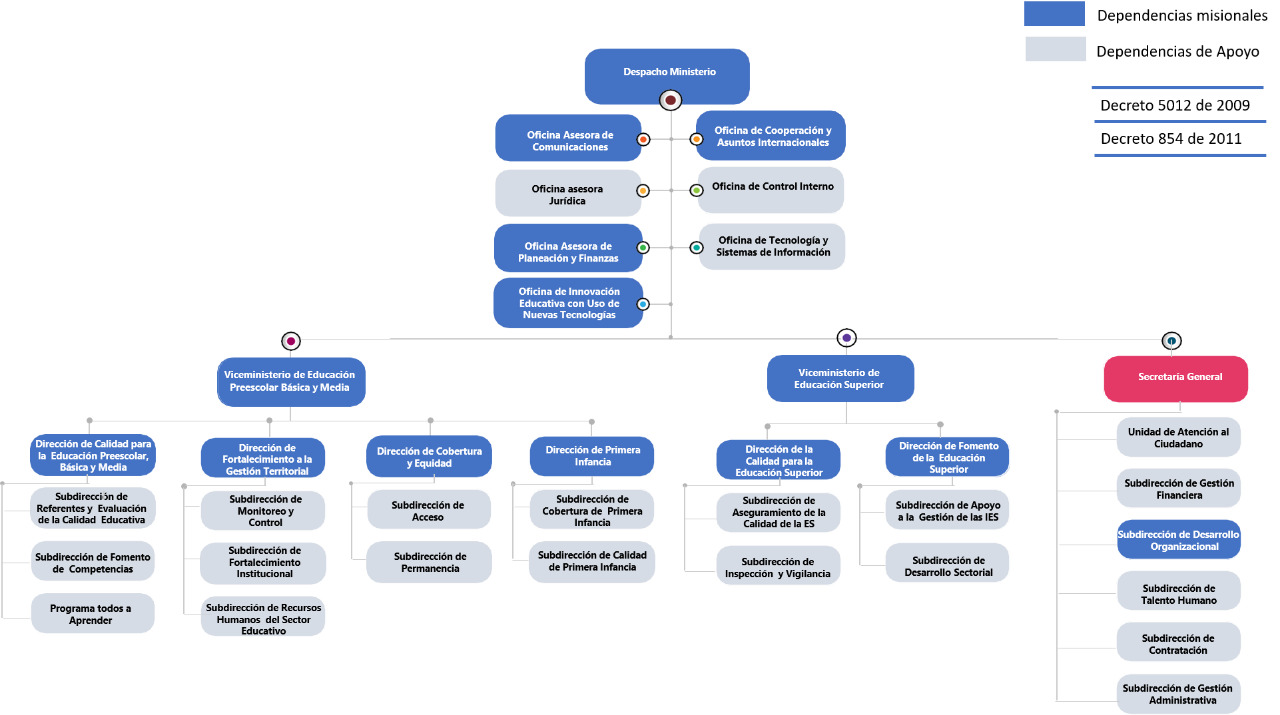
\includegraphics[width=1.1\linewidth]{imgs/organigrama.jpeg}
	\caption{Organigrama MEN}
\end{figure}


\section{Procesos}

\textbf{Procesos Estratégicos:}
\begin{itemize}
	\item Establecer el direccionamiento estratégico sectorial e institucional mediante la formulación y seguimiento de los planes, programas y proyectos, la gestión de la información del sector educación y la asignación de recursos financieros para dar cumplimiento a los objetivos institucionales y sectoriales.
	\item Administrar y mejorar el Sistema Integrado de Gestión, mediante el cumplimiento de los requisitos de los modelos referenciales en concordancia con el contexto estratégico de la entidad y una estructura organizacional que responda a las necesidades de modernización para posicionar el Ministerio de Educación como una entidad ejemplar en materia de gestión y desempeño.
	\item Realizar la difusión e intercambio oportuno, transparente y eficaz de mensajes e información del MEN con los diferentes grupos de interés, mediante la formulación, diseño y ejecución de planes y estrategias de comunicación, la asesoría en comunicación para la movilización, el relacionamiento y las acciones de divulgación y de sensibilización, CON EL FIN de promover la transparencia de la gestión institucional y el posicionamiento del Ministerio.
	\item Establecer alianzas estratégicas internacionales, nacionales, públicas y/o privadas, mediante la búsqueda de aliados, para la gestión de recursos técnicos, políticos, financieros e institucionales que contribuyan al logro de los objetivos misionales del MEN.
	\item Gestionar los recursos de tecnología de la información y las comunicaciones como un factor estratégico generador de valor para la Entidad y el sector educación, mediante la adopción del marco legal para el estado colombiano en materia de TIC, con el fin que las estrategias y proyectos adoptados faciliten a los usuarios el acceso, el uso eficiente y el aprovechamiento de las TIC.
	\item Capitalizar el conocimiento clave del Ministerio mediante su identificación, creación, disposición y socialización, para contribuir al aprendizaje organizacional y la innovación en la prestación de servicios y la ejecución de los procesos.
\end{itemize}

\textbf{Procesos Misionales:}

\begin{itemize}
	\item Diseñar la política pública de educación y sus instrumentos, mediante la identificación de necesidades del país en esta materia y la definición de líneas estratégicas de desarrollo que contribuyan a hacer de Colombia la mejor educada.
	\item Garantizar el logro de los objetivos y metas propuestos en materia de educación, mediante el desarrollo de actividades relacionadas con la ejecución de programas y proyectos, la prestación del servicio de asistencia técnica, el aseguramiento de la calidad y monitoreo, para lograr una educación de calidad eficiente y pertinente.
	\item Definir los lineamientos a tener en cuenta dentro del Ministerio de Educación Nacional cuando se requiera evaluar una política, programa, plan, proyecto, estrategia, acción o un instrumento de política de educación.
	\item Brindar atención a las partes interesadas del MEN, mediante respuestas de calidad, pertinentes y oportunas de las PQRSD, trámites y servicios, a través de canales de comunicación institucionales, con el fin de favorecer la satisfacción de las partes interesadas.
\end{itemize}

\textbf{Procesos de evaluación:}
\begin{itemize}
	\item Evaluar objetiva e independientemente la eficacia, eficiencia y efectividad del sistema integrado de gestión, mediante el desarrollo y seguimiento de las actividades previstas, para fortalecer el autocontrol, la autorregulación y la autogestión del MEN, de conformidad con la normatividad vigente.
	\item Ejercer el control interno disciplinario mediante el cumplimiento de los requisitos normativos.
\end{itemize}

\section{Servicios}

\begin{itemize}
	\item \textbf{Asistencia técnica:} Actividades que se ejecutan para transferir el conocimiento, fortalecer capacidades y desarrollar competencias que propicien prácticas de buen gobierno, faciliten la implementación de la política y mejoren la prestación del servicio educativo, en condiciones de eficiencia, calidad y pertinencia; mediante mecanismos o estrategias de capacitación, asesoría, acompañamiento presencial o virtual, entre otros.
	\item \textbf{Evidencias documentales de asistencia técnica:} Actas de visita o de reunión, listados de asistencia, correos electrónicos, comunicaciones de respuesta a inquietudes, que dan cuenta de que los temas cubrieron las necesidades identificadas y los compromisos objeto de seguimiento por parte del Ministerio de Educación Nacional.
	\item \textbf{Proyectos Ejecutados:} Proyectos Ejecutados en el Ministerio de Educación Nacional, donde se tienen en cuenta los resultados de estos y el impacto en la población objetivo.
	\item \textbf{Trámite de aseguramiento de la calidad:} Hace referencia a los diferentes trámites que se realizan en el Ministerio de Educación Nacional los cuales son: 1 Autorización de creación de seccionales de instituciones de educación superior, 2 Certificación de existencia y representación legal de instituciones de educación superior, 3 Certificación de programa académico de instituciones de educación superior, 4 Redefinición para el Ofrecimiento de Programas por Ciclos Propedéuticos, 5 Reconocimiento de Personería Jurídica de las instituciones de educación superior privadas, 6 Reconocimiento como Universidad de una institución universitaria o escuela tecnológica privada u oficial, 7 Ratificación de reformas estatutarias para institución de educación superior privada, 8 Registro e inscripción de rectores y representantes legales de institución de educación superior IES, 9 Registro calificado, 10 Convalidación de estudios de preescolar, básica y media realizados en el exterior, 11 Certificado de idoneidad del título de postgrado para ascender al grado 14 del escalafón, 12 Convalidación de títulos de estudios de pregrado otorgados en el exterior, 13 Acreditación de alta calidad de Programa Académico de Institución de Educación Superior, 14 Aprobación del estudio de factibilidad socioeconómica en la creación de instituciones de educación superior estatales u oficiales, 15 Legalización de documentos de educación superior para adelantar estudios o trabajar en el exterior, 16 Convalidación de títulos de estudios de posgrado obtenidos en el exterior, 17 Cambio de carácter académico. 18. Reconocimiento de intérpretes oficiales de lengua de señas colombiana - español. 19. Convocatoria beca ser.
	\item \textbf{Apertura de investigación:} Acto administrativo que pone de manifiesto la existencia o comisión de los actos constitutivos de falta administrativa señalados en esta ley.
	\item \textbf{Respuesta a Peticiones, Quejas, Reclamos, Sugerencias - PQRS:} Comunicación realizada al peticionario dando respuesta a la Petición, Queja, Reclamo, Sugerencia - PQRS interpuesta.
	\item \textbf{Atención a la ciudadanía:} Atención prestada por los canales de atención de la Unidad de Atención al Ciudadano del Ministerio de Educación Nacional (presencial, telefónica, chat).
\end{itemize}

\section{Productos}
\begin{itemize}
	\item \textbf{Documento de política pública en educación:} Documentos de política pública en educación: Leyes, Decretos, Conpes, Actos Administrativos, documentos de directrices o lineamientos de política pública en Educación.
	\item \textbf{Documento mediante el cual se establece un instrumento de política pública en educación:} Documentos mediante los cuales se establecen instrumentos de política pública en educación: Actos administrativos, guías, manuales, documentos de directrices, lineamientos, metodologías sobre instrumentos de política pública en Educación. Los tipos de instrumentos de política se encuentran definidos en el Proceso Diseño de Política e Instrumentos de Política del Ministerio de Educación Nacional.
	\item \textbf{Documento de evaluación de política pública o de instrumentos de política pública en educación:} Documento de evaluación de política pública o de instrumentos de política pública en educación. 
	\item \textbf{Video juego para aprender inglés desde casa:} Aplicación digital de nombre \#BThe1Challenge, con la finalidad de ayudar a las personas en el proceso de aprender inglés y de una forma lúdica e interactiva, es un videojuego educativo descargable en tabletas y celulares Android, desarrollado por el Programa Nacional de Bilingüismo de la cartera, en compañía del British Council, con el fin de que "los estudiantes tengan más herramientas de aprendizaje durante el desarrollo de sus actividades académicas no presenciales". El juego está diseñado 100\% en inglés, dirigido a estudiantes de grados 6. ° a 11. ° de instituciones educativas oficiales del país. Estos podrán acceder a la aplicación descargándola a través de la tienda Google Play Store. La idea es que, ya inscritos en el juego, recuperen los objetos ocultos por una fórmula creada por la científica y filántropa Margaret Winter, quien es el personaje creado para esta historia.
\end{itemize}

\section{Requerimientos}
contenido...

\section{Valores Corporativos}
Los Valores del Ministerio de Educación Nacional son las formas de ser y de actuar de los servidores públicos y colaboradores, los cuales se consideran altamente deseables como atributos o cualidades suyas, por cuanto posibilitan la aplicación de los principios éticos y el cabal cumplimiento de los mandatos constitucionales y legales en su desempeño laboral. Los valores del Ministerio son: 


\textbf{Compromiso:} \\
Consciencia de la importancia del rol como servidor público y disposición permanente para comprender y resolver las necesidades de las personas con las que se comparten las labores cotidianas, buscando siempre mejorar su bienestar. \\

\textbf{Lo que hago: }
\begin{itemize}
	\item Atiendo con amabilidad, igualdad y equidad a todas las personas en cualquier situación a través de mis palabras, gestos y actitudes, sin importar su condición social, económica, religiosa, étnica o de cualquier otro orden. Soy amable todos los días, esa es la clave, siempre.
	\item Siempre estoy dispuesto a ponerme en los zapatos de las personas. Entender su contexto, necesidades y requerimientos es el fundamento de mi servicio y labor. 
	\item Escucho, atiendo y oriento a quien necesite cualquier información o guía en algún asunto público. 
	\item Estoy atento siempre que interactúo con otras personas, sin distracciones de ningún tipo. 
\end{itemize}

\textbf{Lo no que hago: }
\begin{itemize}
	\item Trabajar con una actitud negativa. No se vale afectar mi trabajo por no ponerle ganas a las cosas. 
	\item Pensar que mi trabajo como servidor es un “favor” que le hago a la ciudadanía. Es un compromiso y un orgullo. 
	\item Asumir que mi trabajo como servidor es irrelevante para la sociedad.
	\item Ignorar a un ciudadano y sus inquietudes. 
\end{itemize}

El elemento característico de la cultura del MEN que refleja el compromiso es la “Conexión”. \\

\textbf{Honestidad: } \\
Actuar siempre con fundamento en la verdad, cumpliendo los deberes con transparencia y rectitud, favoreciendo el interés general. \\

%\newpage
\textbf{Lo que hago: }
\begin{itemize}
	\item Siempre digo la verdad, incluso cuando cometo errores, porque es humano cometerlos, pero no es correcto esconderlos. 
	\item Cuando tengo dudas respecto a la aplicación de mis deberes busco orientación en las instancias pertinentes al interior de mi entidad. Se vale no saberlo todo, y también se vale pedir ayuda. 
	\item Facilito el acceso a la información pública completa, veraz, oportuna y comprensible a través de los medios destinados para ello.  
	\item Denuncio las faltas, delitos o violación de derechos de los que tengo conocimiento en el ejercicio de mi cargo, siempre. 
	\item Apoyo y promuevo los espacios de participación para que los ciudadanos hagan parte de la toma de decisiones que los afecten relacionadas con mi cargo o labor.  
\end{itemize}

\textbf{Lo no que hago: }
\begin{itemize}
	\item Dar trato preferencial a personas cercanas para favorecerlos en un proceso, porque debe prevalecer la igualdad de condiciones. 
	\item Aceptar incentivos, favores, y cualquier otro tipo de beneficio que me ofrezcan personas o grupos que estén interesados en un proceso de toma de decisiones. 
	\item Usar recursos públicos para fines personales relacionados con mi familia, mis estudios y mis pasatiempos (esto incluye el tiempo de mi jornada laboral, los elementos y bienes asignados para cumplir con mi labor, entre otros). 
	\item Ser descuidado con la información a mi cargo, o con su gestión. 
\end{itemize}

El elemento característico de la cultura del MEN que refleja la honestidad y el respeto es la “Comunicación”. \\

\textbf{Diligencia: } \\
Cumplimiento de los deberes, funciones y responsabilidades asignadas de la mejor manera posible, con atención, prontitud y eficiencia, para así optimizar el uso de los recursos del Estado. \\

%\newpage
\textbf{Lo que hago: }
\begin{itemize}
	\item Uso responsablemente los recursos públicos para cumplir con mis obligaciones. Lo público es de todos y no se desperdicia. 
	\item Cumplo con los tiempos estipulados para el logro de cada obligación laboral. A fin de cuentas, el tiempo de todos es oro. 
	\item Aseguro la calidad en cada uno de los productos que entrego bajo los estándares del servicio público. No se valen cosas a medias. 
	\item Aseguro la calidad en cada uno de los productos que entrego bajo los estándares del servicio público. No se valen cosas a medias. 
\end{itemize}

\textbf{Lo no que hago: }
\begin{itemize}
	\item Malgastar el recurso público. 
	\item Postergar las decisiones y actividades que den solución a problemáticas ciudadanas o que hagan parte del funcionamiento de mi cargo. Hay cosas que sencillamente no se dejan para otro día. 
	\item Demostrar desinterés en mis actuaciones ante los ciudadanos y los demás servidores públicos. 
	\item Evadir mis funciones y responsabilidades. 
	\item Trasladar los problemas y responsabilidades a otras dependencias, siempre aporto a la solución.
\end{itemize}


\textbf{Justicia: } \\
Actuar con imparcialidad, garantizando los derechos de las personas, con equidad, igualdad y sin discriminación. 

\textbf{Lo que hago: }
\begin{itemize}
	\item Tomo decisiones informadas y objetivas basadas en evidencias y datos confiables. Es muy grave fallar en mis actuaciones por no tener las cosas claras. 
	\item Reconozco y protejo los derechos de cada persona de acuerdo con sus necesidades y condiciones. 
	\item Tomo decisiones estableciendo mecanismos de diálogo y concertación con todas las partes involucradas.  
\end{itemize}

\textbf{Lo no que hago: }
\begin{itemize}
	\item Promover y ejecutar políticas, programas o medidas que afectan la igualdad y la libertad de personas. 
	\item Favorecer el punto de vista de un grupo de interés sin tener en cuenta a todos los actores involucrados en una situación. 
	\item Permitir que odios, simpatías, antipatías, caprichos, presiones o intereses de orden personal o grupal interfieran en mi criterio, toma de decisión y gestión pública. 
	\item Dar un trato inequitativo a nuestros usuarios y prelaciones indebidas para favorecer alguna persona. 
\end{itemize}

El elemento característico de la cultura del MEN que refleja la diligencia y la justicia es el “Servicio”. \\

\textbf{Mística: } \\
Actuar con sentido y amor por lo que hacemos. Amor al trabajo, a la Entidad, a los compañeros y a los superiores, propendiendo por un ambiente integro. \\

\textbf{Lo que hago: }
\begin{itemize}
	\item Desarrollo mis actividades con pasión entusiasta.  
	\item Reflejo lo mejor de mí en cada labor.  
	\item Busco trascender en los demás y dar un valor agregado. 
	\item Tengo sentido de pertenencia. 
\end{itemize}

\textbf{Lo no que hago: }
\begin{itemize}
	\item Actuar de manera desinteresada por el logro de los objetivos. 
	\item Falta de escucha y de no conocer las personas, personalidades y desconocer el bien común.
\end{itemize}

\textbf{Confianza: } \\
Creer en los demás, confiar en nuestro trabajo y en nuestros grupos de interés. \\

%\newpage
\textbf{Lo que hago: }
\begin{itemize}
	\item Tengo la certeza de cómo lograremos el cumplimiento de las metas. 
	\item Genero un ambiente de trabajo basado en la apertura, escucha y comunicación.  
	\item Actúo confiado en pro de los objetivos del equipo y/o de la Entidad.  
\end{itemize}

\textbf{Lo no que hago: }
\begin{itemize}
	\item Generar incertidumbre faltando a la verdad y afectando la toma de decisiones. 
	\item Atentar contra los principios de credibilidad de los procesos a cargo. 
	\item Actuar con inseguridad, resistencia y temor a los cambios.
\end{itemize}

\section{Principios Corporativos}

\textbf{Principios de Integridad} \\
En el marco de la Integridad Pública, los servidores del Ministerio de Educación Nacional asumen los siguientes principios de Integridad: 

\begin{enumerate}
	\item El interés general prevalece sobre el interés particular. 
	\item Los bienes y recursos públicos están destinados exclusivamente para asuntos de interés general. 
	\item  La función primordial del servidor público es servir a la ciudadanía. 
	\item Quien administra recursos públicos rinde cuentas a la sociedad sobre su utilización y los resultados de su gestión.
	\item . Los ciudadanos tienen derecho a participar en las decisiones públicas que los afecten.
\end{enumerate}

\chapter{Metodología}
\section{Introducción}

El Método de Desarrollo de la Arquitectura de TOGAF (ADM) forma el núcleo del TOGAF.  Es un método fiable y de eficacia probada para desarrollar una arquitectura de TI que satisfaga las necesidades comerciales de una organización, utilizando los demás elementos de TOGAF, y otros activos arquitectónicos disponibles para la organización. \\

El TOGAF consta de dos partes principales:

\begin{itemize}
	\item    El Método de Desarrollo de la Arquitectura de TOGAF (ADM).
	\item La Arquitectura de la Fundación TOGAF, la cual se trata de una arquitectura de servicios y funciones genéricas que proporciona una base firme sobre la que se pueden construir arquitecturas y componentes arquitectónicos más específicos.
\end{itemize}

La ADM de la TOGAF describe el proceso de pasar de la Arquitectura de la Fundación TOGAF a una arquitectura específica de la organización (o conjunto de arquitecturas), aprovechando los elementos de la Arquitectura de la Fundación TOGAF y otros componentes arquitectónicos y bloques de construcción pertinentes a lo largo del camino.\\

La Arquitectura de la Fundación TOGAF no es, por supuesto, el único recurso disponible para el arquitecto en el uso de la ADM. Hay una amplia gama de modelos arquitectónicos, componentes y bloques de construcción relacionados con diferentes aspectos del dominio de la arquitectura. Este contexto mucho más amplio en el que reside la Arquitectura de la Fundación TOGAF se denomina en la TOGAF el Continuo Empresarial.\\

Es importante señalar que, al ejecutar la ADM, el arquitecto no sólo está desarrollando el resultado final de una arquitectura específica de la organización, sino que también está poblando el propio Continuo Empresarial de la organización, con todos los activos arquitectónicos identificados y apalancados a lo largo del camino - incluyendo, pero no limitado a, la arquitectura específica de la organización resultante.\\

Aunque el enfoque principal de la ADM está en el desarrollo de la arquitectura específica de la organización, en este contexto más amplio la ADM también puede verse como el proceso de poblar el Continuo Empresarial de la organización con bloques de construcción reutilizables relevantes.\\

El desarrollo de la arquitectura es un proceso iterativo y continuo, y al ejecutar la ADM repetidamente a lo largo del tiempo, el arquitecto va poblando gradualmente más y más el Continuo Empresarial de la organización.\\

De hecho, la primera ejecución del ADM será a menudo la más difícil, ya que los activos arquitectónicos disponibles para su reutilización serán relativamente pocos. Sin embargo, las ejecuciones posteriores serán más fáciles, ya que cada vez se identifican más activos de arquitectura, que se utilizan para poblar el Enterprise Continuum de la organización y, por lo tanto, están disponibles para su reutilización.

\newpage
\section{ADM}
\begin{figure}[h!]
	\centering
	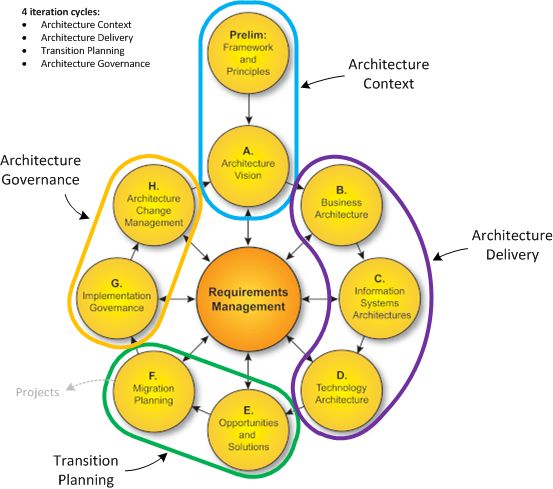
\includegraphics[width=1\linewidth]{imgs/adm.png}
	\caption{ADM \cite{archi3.1,a1,a2,a3,a4}}
\end{figure}

\part{ARQUITECURA}
\chapter{Lenguaje: ArchiMate}
\section{Introducción}
Para el desarrollo de proyectos de ingeniería de software se requiere una serie de componentes, pasos y estructura bien definida que debe seguirse para llevar a buen término la finalización del mismo. Una de estas partes fundamentales en la ingeniería de software es el lenguaje de modelado, el cual es un lenguaje artificial que puede ser utilizado para expresar la información o el conocimiento o sistemas en una estructura que se define por un conjunto coherente de normas. Las reglas se utilizan para interpretar el significado de los componentes de la estructura. Estos lenguajes de modelado pueden ser de dos tipos en específico, el primero es el gráfico, el cual utiliza una técnica de diagrama con símbolos con nombre que representan conceptos y líneas que conectan los símbolos y representan relaciones y varias otras notaciones gráficas para representar restricciones. y el lenguaje textual que puede usar palabras clave estandarizadas acompañadas de parámetros o términos y frases en lenguaje natural para hacer expresiones interpretables por computadora. Entre estos lenguajes de modelado se encuentra uno muy útil el cual es ArchiMate, el cual consiste en un amplio, abierto e independiente lenguaje de modelado con el fin de apoyar la descripción, análisis y visualización de la arquitectura deentro del proyecto de fóma veráz y efectiva. ArchiMate es un estándar técnico de The Open Group y se basa en los conceptos del estándar IEEE 1471 . Cuenta con el respaldo de varios proveedores de herramientas y empresas consultoras. ArchiMate también es una marca registrada de The Open Group. Open Group tiene un programa de certificación para usuarios de ArchiMate, herramientas de software y cursos. ArchiMate se distingue de otros lenguajes como el Lenguaje de modelado unificado (UML) y el Modelado y notación de procesos de negocio (BPMN) por su alcance de modelado empresarial.

\begin{figure}[h!]
	\centering
	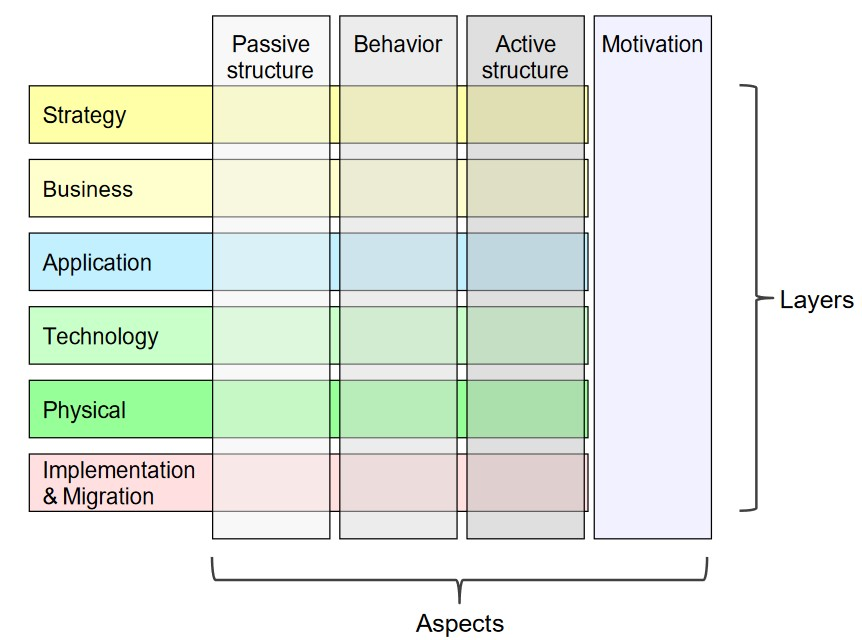
\includegraphics[width=0.7\linewidth]{imgs/coreFramwork}
	\caption{Marco completo de ArchiMate}
\end{figure}

\section{Conceptos y su notación}
El lenguaje ArchiMate separa los conceptos del lenguaje (es decir, los constituyentes del metamodelo) de su notación. Diferentes grupos de interesados pueden requerir diferentes notaciones para comprender un modelo o una visión de la arquitectura.  A este respecto, los ArchiMatelanguages de lenguajes como el UML o el BPMN, que sólo tienen una notación normalizada. El mecanismo de punto de vista explicado en el Capítulo 14 proporciona los medios para definir tales visualizaciones orientadas a las partes interesadas. Aunque la notación de los conceptos de ArchiMate puede (y debería) ser específica de las partes interesadas, la norma proporciona una notación gráfica común, que puede ser utilizada por los arquitectos y otros que desarrollan modelos ArchiMate. Esta notación está dirigida a un público acostumbrado a las técnicas de modelización técnica existentes, como ERD, UML o BPMN, y por lo tanto se asemeja a ellas. En el resto de este documento, a menos que se indique lo contrario, los símbolos utilizados para representar los conceptos del lenguaje representan la notación estándar de ArchiMate.  Esta notación estándar para la mayoría de los elementos consiste en un cuadro con un icono en la esquina superior derecha. En varios casos, este icono por sí mismo puede también utilizarse como notación alternativa. Esta iconografía estándar debe preferirse siempre que sea posible para que cualquier persona que conozca el lenguaje ArchiMate pueda leer los diagramas producidos en el lenguaje.

\subsection{Meta}

La principal jerarquía de elementos de comportamiento y estructura del lenguaje ArchiMate se presenta en la tabla 3.1. Define estos elementos de forma genérica e independiente de la capa. Nótese que la mayoría de estos elementos (las cajas blancas) son elementos abstractos del metamodelo; es decir, no están instanciados en los modelos sino que sólo sirven para estructurar el metamodelo.  La notación presentada es, por lo tanto, la forma genérica en que se representan las especializaciones de estos elementos (es decir, los elementos de las diferentes capas de la arquitectura). Además de describir  los elementos concretos (los recuadros grises), que pueden utilizarse para modelar la Arquitectura de la Empresa a nivel estratégico.

\newpage
\subsubsection{Elementos de la Estructura}
	\begin{table}[h!]
	\begin{tabular}{| m{7em} | m{7cm} | m{3cm} |}
		\hline
		Concepto & Descripción & Representación \\
		
		\hline
		Motivación
		& 
		Un elemento de motivación representa el contexto o la motivación detrás de la  arquitectura de la empresa
		& 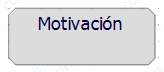
\includegraphics[width=0.8\linewidth, height=0.05\textheight]{imgs/conceptos/meta/Motivacion}
		\\
		
		\hline
		Estructura 
		& 
		Elementos de estructura son equivalentes sinónimos, se subdividen  en estructuras activas ,                              estructuras activas internas,  estructuras activas externas y estructuras pasivas
		& 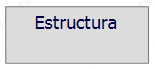
\includegraphics[width=0.8\linewidth, height=0.05\textheight]{imgs/conceptos/meta/Estructura}
		\\
		
		\hline
		Estructura activa  
		& 
		Estructuras que pueden tener un comportamiento
		& 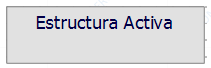
\includegraphics[width=0.8\linewidth, height=0.05\textheight]{imgs/conceptos/meta/EstructuraActiva}
		\\  
		
		\hline
		Estructura activa externa  
		& 
		Llamado interfase representa un punto de acceso donde uno o mas servicios son prestados al ambiente  
		&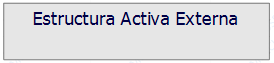
\includegraphics[width=0.8\linewidth, height=0.05\textheight]{imgs/conceptos/meta/EstructuraActivaExterna}
		\\
		
		\hline
		Estructura activa interna
		& 
		Es un elemento que representa una entidad que es capaz de mostrar comportamiento
		& 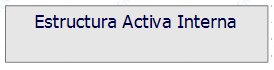
\includegraphics[width=0.8\linewidth, height=0.05\textheight]{imgs/conceptos/meta/EstructuraActivaInterna.PNG}
		\\
		
		\hline
		Estructura pasiva
		& 
		Es un elemento que representa una entidad sobre la cual se realiza un comportamiento
		& 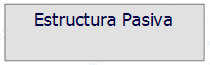
\includegraphics[width=0.8\linewidth, height=0.05\textheight]{imgs/conceptos/meta/EstructuraPasiva.PNG}
		\\
		
		\hline
		Interfase
		& 
		Representa un punto de acceso donde uno o mas servicios son puestos en el ambiente.
		& 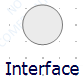
\includegraphics[width=0.8\linewidth, height=0.05\textheight]{imgs/conceptos/meta/Interface.PNG}
		\\
		
		\hline
		
		Comportamiento
		& 
		Es un elemento que equivale a un verbo se  subdivide en evento ,comportamiento interno, proceso , función, interacción, comportamiento externo y servicio.
		& 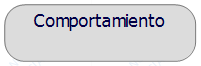
\includegraphics[width=0.8\linewidth, height=0.05\textheight]{imgs/conceptos/meta/Comportamiento.PNG}
		\\
		
		\hline
		Evento
		&
		Representa un cambio de estado 
		& 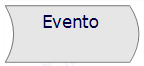
\includegraphics[width=0.8\linewidth, height=0.05\textheight]{imgs/conceptos/meta/Evento.PNG}
		\\
		
		\hline
		Elemento de comportamiento interno 
		& 
		Representa una o mas unidades de actividades que pueden ser realizadas por uno o mas elementos de estructura activa
		& 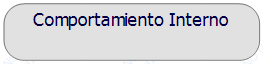
\includegraphics[width=0.8\linewidth, height=0.05\textheight]{imgs/conceptos/meta/ComportamientoInterno.PNG}
		\\	\hline
	\end{tabular}
	%\caption{}
	\label{tab:concepts}
\end{table}

\newpage
\begin{table}[h!]
\begin{center}
	\begin{tabular}{| m{6em} | m{7cm} | m{3cm} |}
		\hline
		Concepto & Descripción & Representación \\ 
		
		\hline
		Servicio
		&
		Un servicio es un comportamiento del sistema proveedor  visible  externamente 
		&
		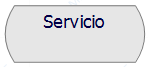
\includegraphics[width=0.8\linewidth, height=0.05\textheight]{imgs/conceptos/meta/Servicio.PNG}
		\\
		
		\hline
		Función
		& 
		Representa una colección de comportamientos, basado en una colección de criterios específicos, tales como fuente requerida, competencias o localización   
		& 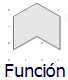
\includegraphics[width=0.8\linewidth, height=0.05\textheight]{imgs/conceptos/meta/Funcion.PNG}
		\\
		
		\hline
		Proceso
		& 
		Representa una secuencia de comportamientos que consiguen un resultado especifico
		& 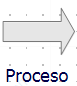
\includegraphics[width=0.8\linewidth, height=0.05\textheight]{imgs/conceptos/meta/Proceso.PNG}
		\\
		
		\hline
		Interacción  
		& 
		Representa una unidad de comportamientos que deben ser realizados por dos o mas elementos de estructura activa interna , ya sea a través de una asignación directa o agregados en una colaboración 
		& 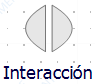
\includegraphics[width=0.8\linewidth, height=0.05\textheight]{imgs/conceptos/meta/Interaccion.PNG}
		\\
		
		\hline
		Colaboración  
		& 
		Representa un acuerdo entre dos o mas elementos estructuras activas internas, trabajan juntos para realizar algún comportamiento colectivo   
		& 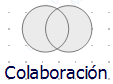
\includegraphics[width=0.8\linewidth, height=0.05\textheight]{imgs/conceptos/meta/Colaboracion.PNG}
		\\
		
		\hline
		Elemento de comportamiento externo
		& 
		Representa un comportamiento explicito que es visible en el exterior  
		& 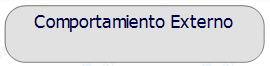
\includegraphics[width=0.8\linewidth, height=0.05\textheight]{imgs/conceptos/meta/ComportamientoExterno.PNG}
		\\
		
		\hline
		
		Elementos compuestos 
		&
		Son elementos que se basan en aspectos de otras capas del lenguaje   
		&
		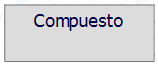
\includegraphics[width=0.8\linewidth, height=0.05\textheight]{imgs/conceptos/meta/Compuesto.PNG}
		\\
		
		\hline
	\end{tabular}
	\caption{Conceptos capa meta}
	\label{tab:concepts}
\end{center}
\end{table}

\newpage
\subsection{Motivación}

Los elementos de motivación se utilizan para modelar las motivaciones, o razones, que guían el diseño o el cambio de una Arquitectura Empresarial. Es esencial entender los factores, a menudo denominados impulsores, que influyen en otros elementos de motivación.  Pueden originarse tanto dentro como fuera de la empresa.  Los impulsores internos, también llamados preocupaciones, están asociados con las partes interesadas, que pueden ser algún ser humano individual o algún grupo de seres humanos, como un equipo de proyecto, una empresa o la sociedad. Ejemplos de esos impulsores internos son la satisfacción del cliente, el cumplimiento de la legislación o la rentabilidad. Es común que las empresas realicen una evaluación de esos factores impulsores; por ejemplo, utilizando un análisis FODA, a fin de responder de la mejor manera posible.

\begin{center}
	\begin{tabular}{ | m{6em} | m{4cm}| m{2cm} | } 
		\hline
		Motivación& Un elemento que proporciona el contexto o la razón detrás de la arquitectura de una empresa & 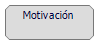
\includegraphics[width=0.8\linewidth, height=0.05\textheight]{imgs/Elementos/Motivacion.PNG}
		\\ 
		\hline
	\end{tabular}
\end{center}

\newpage
\subsubsection{Elementos de la Estructura}
\begin{table}[h!]
	\begin{center}
		\begin{tabular}{| m{6em} | m{7cm}| m{3cm} |}
			\hline
			Concepto & Descripción & Representación \\ 
			\hline
			
			Implicado 
			& 
			El papel de un individuo, equipo u organización (o clases de los mismos) que representa sus intereses en el resultado de la arquitectura 
			& 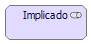
\includegraphics[width=0.8\linewidth, height=0.05\textheight]{imgs/Elementos/Implicado.PNG}
			\\
			\hline
			Manejador 
			& 
			Una condición externa o interna que motiva a una organización para definir sus galones e implementar los cambios necesarios para lograrlos. 
			& 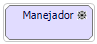
\includegraphics[width=0.8\linewidth, height=0.05\textheight]{imgs/Elementos/Manejador.PNG}
			\\
			\hline
			Valoración 
			& 
			El resultado de un análisis de la situación de la empresa con respecto a algún conductor. 
			& 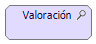
\includegraphics[width=0.8\linewidth, height=0.05\textheight]{imgs/Elementos/Valoracion.PNG}
			\\
			\hline
			Objetivo 
			& 
			Una declaración de intención, dirección o estado final deseado de alto nivel para una organización y sus partes interesadas. 
			& 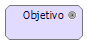
\includegraphics[width=0.8\linewidth, height=0.05\textheight]{imgs/Elementos/Objetivo.PNG}
			\\
			\hline
			Resultado 
			& 
			Un resultado final que se ha logrado
			& 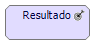
\includegraphics[width=0.8\linewidth, height=0.05\textheight]{imgs/Elementos/Resultado.PNG}
			\\
			\hline
			Principio 
			& 
			Una declaración cualitativa de intenciones que debe ser satisfecha por la arquitectura
			& 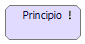
\includegraphics[width=0.8\linewidth, height=0.05\textheight]{imgs/Elementos/Principio.PNG}
			\\
			\hline
			Requerimiento 
			& 
			Una declaración de necesidad que debe ser satisfecha por la arquitectura
			& 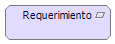
\includegraphics[width=0.8\linewidth, height=0.05\textheight]{imgs/Elementos/Requerimiento.PNG}
			\\
			\hline
			Restricción 
			& 
			Un factor que previene oUn factor que previene u obstruye laUn factor que previene u obstruye la realizaciónUn factor que previene u obstruye la realización de metas
			& 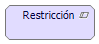
\includegraphics[width=0.8\linewidth, height=0.05\textheight]{imgs/Elementos/Restriccion.PNG}
			\\
			\hline
			Significado 
			& 
			Los conocimientos o la experiencia presentes en, o la interpretación dada a, un elemento
			& 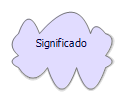
\includegraphics[width=0.8\linewidth, height=0.05\textheight]{imgs/Elementos/Significado.PNG}
			\\
			\hline
			Valor 
			& 
			El valor relativo, la utilidad o la importancia de un elemento básico o un resultado
			& 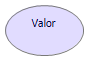
\includegraphics[width=0.8\linewidth, height=0.05\textheight]{imgs/Elementos/Valor.PNG}
			\\
			
			\hline
		\end{tabular}
		\caption{Conceptos Capa Motivacional}
		\label{tab:concepts}
	\end{center}
\end{table}

\subsection{Punto de Vista Estratégico}
Para describir los aspectos de la estrategia de nuestra empresa, se explicaran los siguientes puntos de vista presentado diferentes perspectivas de la aplicación del modelo a la dirección de nuestra empresa:
\subsubsection{Punto de vista de estrategia}
\begin{table}[th!]
	\begin{center}
		\begin{tabular}{| c | p{6cm} |} %r c|}
			\hline
			\multicolumn{2}{ |c| }{Punto de vista de la estrategia}
			
			\\ \hline
			
			Stakeholders
			& 
			CxOs(Chief eXperience Officer), gerentes del negocio y arquitectos empresariales y de negocio. 
			
			\\ \hline
			Ocupaciones 
			& 
			Desarrollador de estrategias.
			
			\\ \hline
			
			Propósito 
			& 
			Desarrollo y toma de decisiones.
			
			\\ \hline
			
			Alcance 
			& 
			Estrategia. 
			
			\\ \hline
			
			Elementos relacionados 
			& 
			Cursos de acción, capacidad, flujo del valor, recurso, Outcomes.     		
			
			\\ \hline
		\end{tabular}
		\caption{Descripción del punto de vista de estrategia}
	\end{center}
\end{table}

\subsubsection{Punto de vista del mapeado de las capacidades}
\par Permite mostrar un punto de vista general de las capacidades de la empresa; típicamente el mapeado nos muestra 2 o 3 niveles de las capacidades de una empresa, por ejemplo se puede crear un mapeado de calor que nos muestre áreas de inversión, además en algunos casos nos permite especificar las salidas con sus determinadas capacidades.
\begin{table}[th!]
	\begin{center}
		\begin{tabular}{| c | p{8cm} |} %r c|}
			\hline
			\multicolumn{2}{ |c| }{mapeado de las capacidades}
			
			\\ \hline
			
			Stakeholders
			& 
			Gerentes del negocio y arquitectos empresariales y de negocio. 
			
			\\ \hline
			Ocupaciones 
			& 
			Arquitecto de estrategias, tácticas y motivación.
			
			\\ \hline
			
			Propósito 
			& 
			Desarrollo y toma de decisiones.
			
			\\ \hline
			
			Alcance 
			& 
			Estrategia. 
			
			\\ \hline
			
			Elementos relacionados 
			& 
			capacidad, recurso, Outcomes.     		
			
			\\ \hline
		\end{tabular}
		\caption{Descripción del punto de vista del mapeado de las capacidades}
	\end{center}
\end{table}

\subsubsection{Punto de vista del flujo del valor}
\par Permite mostrar un punto de vista general del flujo del valor; Identifica las capacidades que soportan las etapas en el flujo del valor, valor creado y stakeholders involucrados.
\begin{table}[th!]
	\begin{center}
		\begin{tabular}{| c | p{8cm} |} %r c|}
			\hline
			\multicolumn{2}{ |c| }{Flujo del valor}
			
			\\ \hline
			
			Stakeholders
			& 
			Gerentes del negocio y arquitectos empresariales y de negocio. 
			
			\\ \hline
			Ocupaciones 
			& 
			Arquitecto de estrategias, tácticas y motivación.
			
			\\ \hline
			
			Propósito 
			& 
			Desarrollo y toma de decisiones.
			
			\\ \hline
			
			Alcance 
			& 
			Estrategia. 
			
			\\ \hline
			
			Elementos relacionados 
			& 
			capacidad, flujo del valor, Outcomes, stakeholders.     		
			
			\\ \hline
		\end{tabular}
		\caption{Descripción del punto de vista del flujo del valor}
	\end{center}
\end{table}

\subsubsection{Punto de vista realización de resultados}
\par Este punto de vista es usado para mostrar el nivel más alto de la arquitectura, muestra los negocios orientados a los resultados producidos por las capacidades y los elementos adyacentes al núcleo de la empresa.
\begin{table}[th!]
	\begin{center}
		\begin{tabular}{| c | p{8cm} |} %r c|}
			\hline
			\multicolumn{2}{ |c| }{Realización de resultados}
			
			\\ \hline
			
			Stakeholders
			& 
			Gerentes del negocio y arquitectos empresariales y de negocio. 
			
			\\ \hline
			Ocupaciones 
			& 
			Negocios orientados a resultados.
			
			\\ \hline
			
			Propósito 
			& 
			Desarrollo y toma de decisiones.
			
			\\ \hline
			
			Alcance 
			& 
			Estrategia. 
			
			\\ \hline
			
			Elementos relacionados 
			& 
			capacidad, flujo del valor, recursos, Outcomes, valor, aceptación, elementos del núcleo.     		
			
			\\ \hline
		\end{tabular}
		\caption{Descripción punto de vista de realización de resultados}
	\end{center}
\end{table}

\subsubsection{Punto de vista mapeado de recursos}
\par Permite crear y estructurar una visión general de los recursos de la empresa; típicamente el mapeado nos muestra 2 o 3 niveles de las capacidades de una empresa, por ejemplo se puede crear un mapeado de calor que nos muestre áreas de inversión, además en algunos casos nos permite especificar las relaciones entre los recursos y las capacidades asignadas.
\begin{table}[th!]
	\begin{center}
		\begin{tabular}{| c | p{8cm} |} %r c|}
			\hline
			\multicolumn{2}{ |c| }{mapeado de recursos}
			
			\\ \hline
			
			Stakeholders
			& 
			Gerentes del negocio y arquitectos empresariales y de negocio. 
			
			\\ \hline
			Ocupaciones 
			& 
			Arquitecto de estrategias, tácticas y motivación.
			
			\\ \hline
			
			Propósito 
			& 
			Desarrollo y toma de decisiones.
			
			\\ \hline
			
			Alcance 
			& 
			Estrategia. 
			
			\\ \hline
			
			Elementos relacionados 
			& 
			capacidad,recursos, paquetes de trabajo.     		
			
			\\ \hline
		\end{tabular}
		\caption{Descripción punto de vista mapeado de recursos}
	\end{center}
\end{table}

\subsection{Negocio}

La Capa de Negocios se utiliza típicamente (en conjunto con los elementos de estrategia) para modelar la arquitectura de negocios de una empresa, definida por el marco del TOGAF como una descripción de la estructura e interacción entre la estrategia de negocios, la organización, las funciones, los procesos de negocios y las necesidades de información.

\subsubsection{Elementos de la Estructura}
\begin{table}[H]
	\centering
	\begin{tabular}{| m{3cm} | m{7cm} | m{3.8cm} |}
		\hline
		\textbf{Concepto}           & \textbf{Definición} & \textbf{Notación} \\ \hline
		
		Actor de Negocios        & Una entidad organizacional que es capaz de ejecutar un comportamiento.                                                                                                              &\vspace{1.52mm}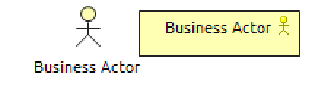
\includegraphics[width=40mm, height=10mm]{imgs/conceptos/negocio/Business_actor.pdf}    \\ \hline
		
		Rol de Negocios          & La responsabilidad de tener un comportamiento especifico, ante el cual un actor puede ser asignado.                                                                                 &\vspace{1.52mm}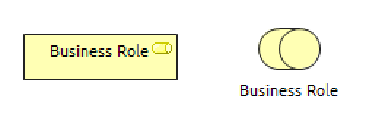
\includegraphics[width=40mm, height=10mm ]{imgs/conceptos/negocio/Business_role.pdf}         \\ \hline
		
		Colaboración de Negocios & Un agregado de dos o más roles de negocios que trabajan juntos para tener un comportamiento colectivo.                                                                             
		&\vspace{1.52mm} 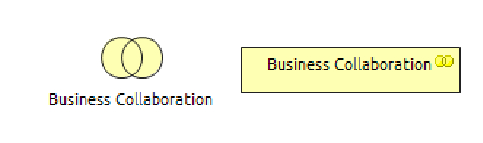
\includegraphics[width=40mm,height=10mm]{imgs/conceptos/negocio/Business_colaboration.pdf}             \\ \hline
		
		Interfaz de Negocios     & Un punto de acceso donde un servicio comercial está disponible para su entorno.                                                                                                     
		&\vspace{1.52mm}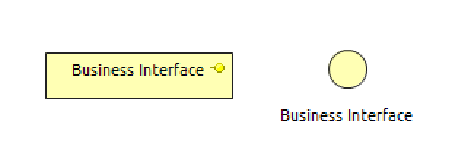
\includegraphics[width=40mm,height=10mm]{imgs/conceptos/negocio/Business_Interface.pdf}  \\ \hline
		
		Ubicación                & Un punto conceptual en el espacio.                                                                                     
		&\vspace{1.52mm}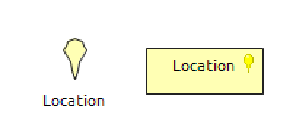
\includegraphics[width=40mm, height=10mm]{imgs/conceptos/negocio/Location.pdf}           \\ \hline
		
		Objeto de Negocios       & Un elemento pasivo que tiene relevancia desde una perspectiva de negocios.                                                                                                         
		&\vspace{1.52mm}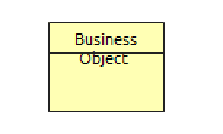
\includegraphics[width=40mm, height=10mm]{imgs/conceptos/negocio/Business_Object.pdf}   \\ \hline
		
		Proceso de Negocios      & Un elemento de comportamiento que agrupa el comportamiento basado en un orden de actividades. Es destinado a producir un  conjunto definido de productos o servicios comerciales.
		&\vspace{1.52mm} 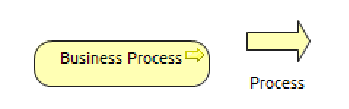
\includegraphics[width=40mm, height=10mm]{imgs/conceptos/negocio/Business_proces.pdf}            \\ \hline
		
		Función de Negocios      & Un elemento de comportamiento que agrupa el comportamiento basado en un conjunto de criterios elegidos (típicamente recursos comerciales requeridos y / o competencias).        &\vspace{1.52mm}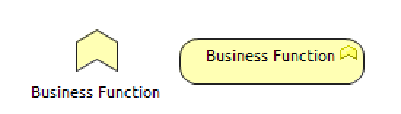
\includegraphics[width=40mm, height=10mm]{imgs/conceptos/negocio/Business_function.pdf}            \\ \hline
		
		Interacción de Negocios  & Un elemento de comportamiento que describe la conducta de una colaboración empresarial.                                                                                             
		&\vspace{1.52mm} 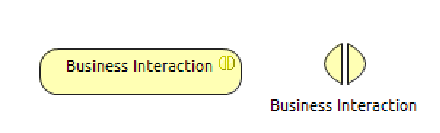
\includegraphics[width=40mm,height=10mm]{imgs/conceptos/negocio/Business_interaction.pdf}            \\ \hline
		
		Evento de Negocios       & Algo que sucede (internamente o externamente) e influye en el  comportamiento.                                                                                                       
		&\vspace{1.52mm} 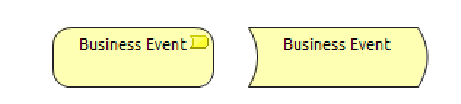
\includegraphics[width=40mm, height=10mm]{imgs/conceptos/negocio/Business_event.pdf}  \\ \hline
		
	\end{tabular}
\end{table}

\newpage
\begin{table}[H]
	\centering
	\begin{tabular}{| m{3cm} | m{7cm} | m{3.8cm} |}
		\hline
		\textbf{Concepto}           & \textbf{Definición} & \textbf{Notación} \\ \hline
		
		Servicio de Negocios     & Un servicio que satisface una necesidad comercial de un cliente (interno o externo al organización).        &\vspace{2mm}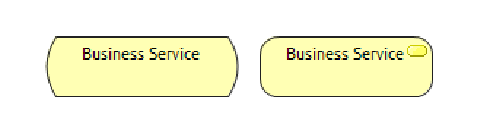
\includegraphics[width=40mm, height=8mm]{imgs/conceptos/negocio/Business_service.pdf}  \\ \hline
		
		Representación           & Una forma perceptible de la información llevado por un objeto de negocios.                                                                                                           &\vspace{1.52mm}  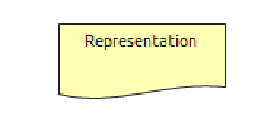
\includegraphics[width=40mm, height=10mm]{imgs/conceptos/negocio/Representation.pdf}            \\ \hline
		Significado              & El conocimiento o experiencia presente en un objeto de negocios o su representación, dado un contexto particular.                                                                   &\vspace{1.52mm}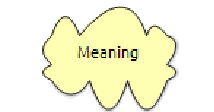
\includegraphics[width=40mm, height=8mm]{imgs/conceptos/negocio/Meaning.pdf}           \\ \hline
		
		Valor                    & El valor relativo, la utilidad o la importanciade un servicio o producto comercial.                                                                                                  
		&\vspace{1.52mm}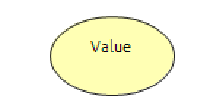
\includegraphics[width=40mm, height=10mm]{imgs/conceptos/negocio/Value.pdf}        \\ \hline
		
		Producto                 & Una colección coherente de servicios, acompañado de un contrato / conjunto de acuerdos, que se ofrece en su conjunto para (internos o externos) clientes.                           &\vspace{1.52mm}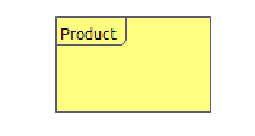
\includegraphics[width=40mm, height=10mm]{imgs/conceptos/negocio/Product.pdf}         \\ \hline
		
		Contrato                 & Una especificación formal o informal de acuerdo que especifica los derechos y obligaciones asociadas con un producto.                                                                 &\vspace{1.52mm}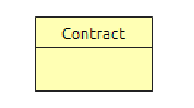
\includegraphics[width=40mm, height=10mm]{imgs/conceptos/negocio/Contract.pdf}       \\ \hline
		
	\end{tabular}
\end{table}

\subsection{Punto de Vista de la Aplicación}
El punto de vista de Aplicación describe el comportamiento interno de una aplicación; por ejemplo, cuando realiza uno o más servicios de aplicación.

\subsubsection{Punto de Vista de comportamiento}
Este punto de vista es útil para diseñar el comportamiento principal de las aplicaciones o para identificar la superposición funcional entre diferentes aplicaciones. Se preocupa por la estructura, relaciones y dependencias entre aplicaciones, consistencia e integridad, reducción de complejidad de la aplicación
\begin{figure}[th!]
	\centering
	\fcolorbox{black}{white}{
		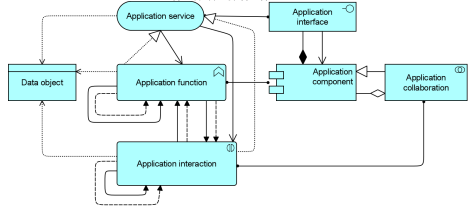
\includegraphics[width=0.9\linewidth]{imgs/puntos_vista/aplicacion/vistacomportamiento}}
	\caption{vista de comportamiento de aplicación}
	\label{fig:vistaaplicacion}
\end{figure}

\subsubsection{Punto de Vista de cooperacion}
El punto de vista de la cooperación de aplicaciones describe las relaciones entre los componentes de las aplicaciones en términos de los flujos de información entre ellos, o en términos de los servicios que ofrecen y utilizan. Este punto de vista se utiliza normalmente para crear una descripción general del panorama de aplicaciones de una organización. Este punto de vista también se utiliza para expresar la cooperación interna o la orquestación de servicios que en conjunto apoyan la ejecución de un proceso empresarial.

\begin{figure}[th!]
	\centering
	\fcolorbox{black}{white}{
		\includegraphics[width=0.9\linewidth]{imgs/puntos_vista/aplicacion/vistacooperacion}}
	\caption{vista de cooperacion de aplicación}
	\label{fig:vistaaplicacion}
\end{figure}

\subsubsection{Punto de Vista de estructura}
El punto de vista Estructura de la aplicación muestra la estructura de una o más aplicaciones o componentes. 
Este punto de vista es útil para diseñar o comprender la estructura principal de aplicaciones o componentes y los datos asociados; p. ej., para desglosar la estructura del sistema en construcción o para identificar componentes de aplicaciones heredados que son adecuados para la migración / integración
\begin{figure}[th!]
	\centering
	\fcolorbox{black}{white}{
		\includegraphics[width=0.9\linewidth]{imgs/puntos_vista/aplicacion/vistaestructura}}
	\caption{vista de estructura de aplicación}
	\label{fig:vistaaplicacion}
\end{figure}	

\subsubsection{Punto de Vista de uso}
El punto de vista Uso de aplicaciones describe cómo se utilizan las aplicaciones para dar soporte a uno o más procesos de negocio y cómo las utilizan otras aplicaciones. 
Se puede utilizar para diseñar una aplicación identificando los servicios que necesitan los procesos de negocio y otras aplicaciones, o para diseñar procesos de negocio al describir los servicios que están disponibles. 

\subsection{Punto de Vista de la Tecnología}
El punto de vista de infraestructura general, trata acerca del hardware y la infraestructura de comunicación que soporta la capa de aplicación. Esta capa ofrece servicios de infraestructura requeridos para desplegar las aplicaciones realizadas en los ordenadores y los sistemas de
hardware y software.



\subsubsection{Punto de vista de uso de infraestructura}

El punto de vista de uso de infraestructura muestra como las aplicaciones son soportadas por la infraestructura de software y hardware: los servicios de infraestructura son entregados por los dispositivos, los sistemas de software y redes son entregados a las aplicaciones. Este
punto de vista juega un rol importante en el análisis del rendimiento y la escalabilidad y puede ser usado para determinar requerimientos de rendimiento y calidad en la infraestructura basado en las demandas de las aplicaciones que la usan.
\newpage

\begin{figure}[h]
	\centering
	\fcolorbox{black}{white}{
		\includegraphics[width=0.5\linewidth]{imgs/puntos_vista/tecnologia/MMDUDI.jpg}}
	\caption{Metamodelo de uso de infraestructura}
\end{figure}

\subsubsection{Modelo de uso de infraestructura}

En este punto de vista se identifican los servicios de infraestructura principales que corresponden al servicio de notificaciones, generar reportes, establecer tiempos de acceso a la
aplicación, y gestionar los usuarios. Cada uno de los servicios de infraestructura entrega configuración y la funcionalidad requerida hacia los componentes de aplicación.


\begin{figure}[h]
	\centering
	\fcolorbox{black}{white}{
		\includegraphics[width=0.5\linewidth]{imgs/puntos_vista/tecnologia/MDUDI.jpg}}
	\caption{Modelo de uso de infraestructura}
\end{figure}



\subsubsection{ Punto de vista de Implementación y despliegue}
El punto de vista de implementación y despliegue muestra como uno o más aplicaciones son realizadas sobre la infraestructura. Esto implica el mapeo de aplicaciones (lógicas) y componentes en artefactos (físicos). Esta vista juega un papel importante en el análisis del rendimiento y la escalabilidad debido a la relación entre la infraestructura y el mundo lógico de las aplicaciones.


\begin{figure}[h]
	\centering
	\fcolorbox{black}{white}{
		\includegraphics[width=0.5\linewidth]{imgs/puntos_vista/tecnologia/MMDIYD.jpg}}
	\caption{Metamodelo de implementación y despliegue}
\end{figure}

\subsubsection{Modelo de implementación y despliegue}

En este punto de vista, se muestra como todos los componentes son realizados por el nodo de servidor de aplicaciones, el componente de comunicación va a ser realizado por el nodo servidor de aplicaciones y tiene una relación de asociación con el nodo servidor de e-mail que
proveerá las configuraciones de software específico para el envío de notificaciones, resultados e información sobre el proceso.

\begin{figure}[h]
	\centering
	\fcolorbox{black}{white}{
		\includegraphics[width=0.5\linewidth]{imgs/puntos_vista/tecnologia/MDIYD.jpg}}
	\caption{Modelo de implementación y despliegue}
\end{figure}



\begin{table}[h]
	\begin{center}
		\begin{tabular}{ | m{7em} | m{8cm}|  } 
			\hline
			Interesados & Arquitectos de infraestructura, gerentes operativos 
			\\
			\hline
			Preocupaciones & Estabilidad, seguridad, dependencias, costos de la infraestructura
			\\
			\hline
			Propósito & Diseñar
			\\
			\hline
			Alcance & Una capa / aspecto múltiple
			\\
			\hline
		\end{tabular}
		\caption{Punto de Vista Tecnología}
		\label{tab:concepts}
	\end{center}
\end{table}

\textbf{Elementos que participan: }
\begin{itemize}
	\item Ubicación
	\item Nodo
	\item Colaboración tecnológica
	\item Dispositivo
	\item Software del sistema
	\item Interfaz tecnológica
	\item Red de comunicacion
	\item Camino
	\item Proceso tecnológico / función / interacción
	\item Servicio de tecnología
	\item Evento tecnológico
	\item Artefacto
\end{itemize}

\subsection{Físico}

Estos se basan en la Capa de Tecnología. No se definen elementos de comportamiento físico separados.  Más bien, los elementos de comportamiento de la Capa de Tecnología (función de la tecnología, proceso, interacción, servicio y evento) se usan para modelar el comportamiento de todos los nodos, incluyendo el equipo físico. Dado que el equipo muy a menudo estará controlado por computadora o tendrá una estrecha relación con la tecnología de la información (piense también en los sensores, Internet de las cosas), su comportamiento puede describirse de manera integral utilizando los conceptos de comportamiento de la tecnología existente.

\newpage
\subsubsection{Elementos de la Estructura}

\begin{longtable}{|c| c| c|}
	\hline
	Concepto & Descripción & Representación \\ \hline
	Facilidad
	&
	\begin{tabular}{p{6cm}p{3cm}}
		Representa un recurso físico que tiene la capacidad de
		facilitar (por ejemplo, albergar o ubicar) el uso de equipos. Por lo general, se utiliza para modelar fábricas, edificios o construcciones al aire libre
	\end{tabular} 
	& \includegraphics[width=0.1\linewidth, height=0.05\textheight]{imgs/conceptos/fisico/facilidad}
	\\
	\hline 
	Equipo
	& 
	\begin{tabular}{p{6cm}p{3cm}}
		El equipo comprende todos los elementos de procesamiento activos que llevan a cabo procesos físicos en los que se utilizan o transforman materiales.
	\end{tabular} 
	& \includegraphics[width=0.1\linewidth, height=0.05\textheight]{imgs/conceptos/fisico/equipo}
	\\
	\hline
	Red de distribución
	&
	\begin{tabular}{p{6cm}p{3cm}} 
		Representa la distribución física o la infraestructura de transporte. Encarna la realización física de las rutas lógicas entre nodos. Una red de distribución conecta dos o más nodos. Una red de distribución puede realizar uno o más caminos.
	\end{tabular} 
	& \includegraphics[width=0.1\linewidth, height=0.05\textheight]{imgs/conceptos/fisico/redDistribucion}
	\\
	\hline
	Material
	&
	\begin{tabular}{p{6cm}p{3cm}}  
		El material representa materia física tangible, con atributos como tamaño y peso. Suele utilizarse para modelar materias primas y productos físicos, y también fuentes de energía como el combustible.
	\end{tabular}
	& \includegraphics[width=0.1\linewidth, height=0.05\textheight]{imgs/conceptos/fisico/material}
	\\
	\hline
\end{longtable}

\section{Relaciones}

el lenguaje ArchiMate define un conjunto básico de relaciones genéricas, cada una de las cuales puede conectar un conjunto predefinido de conceptos de origen y destino (en la mayoría de los casos elementos, pero en unos pocos casos también otras relaciones).  Muchas de estas relaciones están "sobrecargadas"; es decir, su significado exacto difiere según los conceptos de origen y destino que conectan, y se clasifican de la siguiente manera:
\begin{itemize}
	\item Relaciones estructurales, que modelan la construcción o composición estática de conceptos del mismo o diferentes tipos.
	\item Relaciones de dependencia, que modelan cómo se utilizan los elementos para apoyar otros elementos.
	\item Las relaciones dinámicas, que se utilizan para modelar las dependencias de comportamiento entre los elementos.
	\item Otras relaciones, que no entran en ninguna de las categorías anteriores.
\end{itemize}

\subsection{Relaciones Estructurales}

Las relaciones estructurales representan la coherencia "estática" dentro de una arquitectura.  El concepto de composición (el lado "de" de la relación) es siempre un elemento; el concepto de composición (el lado "de" de la relación) puede en algunos casos ser también otra relación.

\begin{table}[h!]
	\subsubsection{Elementos}
	\begin{center}
		\begin{tabular}{| l | l | r |}
			\hline
			Concepto & Descripción & Representación \\ \hline
			
			Agregación 
			&
			\begin{tabular}[l]{@{}l@{}}
				Indica que un elemento consiste en \\
				uno u otros conceptos más.
			\end{tabular}
			& \includegraphics[width=0.4\linewidth]{imgs/relaciones/agregacion}
			\\\hline
			
			Composición
			& 
			\begin{tabular}[l]{@{}l@{}}
				Indica que un elemento consiste en \\
				uno u otros conceptos más.
			\end{tabular}
			& \includegraphics[width=0.4\linewidth]{imgs/relaciones/composicion}
			\\\hline
			
			Asignación
			& 
			\begin{tabular}[l]{@{}l@{}}
				Expresa la asignación de \\
				responsabilidad, la ejecución \\
				de la conducta, o la ejecución.
			\end{tabular}
			& \includegraphics[width=0.4\linewidth]{imgs/relaciones/asignacion}
			\\\hline
			
			Realización
			& 
			\begin{tabular}[l]{@{}l@{}}
				Indica que una entidad desempeña \\
				un papel fundamental en la creación,\\
				el logro, el sustento o el \\
				funcionamiento de una entidad más \\
				abstracta.
			\end{tabular}
			& \includegraphics[width=0.4\linewidth]{imgs/relaciones/realizacion}
			\\\hline
			
		\end{tabular}
		\caption{Relaciones estructurales}
		\label{tab:estructurales}
	\end{center}
\end{table}

\subsection{Relaciones de Dependencia}

Las relaciones de dependencia describen la forma en que los elementos apoyan o son utilizados por otros elementos.  Se distinguen tres tipos de relaciones de dependencia:
\begin{itemize}
	\item La relación de servicio representa una dependencia de control, denotada por una línea sólida.
	\item La relación de acceso representa una dependencia de datos, denotada por una línea discontinua.
	\item La relación de influencia es el tipo de dependencia más débil, utilizada para modelar cómo los elementos de motivación son influenciados por otros elementos.
\end{itemize}
Obsérvese que, aunque la notación de estas relaciones se asemeja a la notación de la relación de dependencia en UML, estas relaciones tienen significados distintos en la notación ArchiMate y (normalmente) apuntan en la dirección opuesta.

\begin{table}[h!]
	\subsubsection{Elementos}
	\begin{center}
		\begin{tabular}{| c | l | l |}
			\hline
			Concepto & Descripción & Representación \\ \hline
			
			Sirve 
			&
			\begin{tabular}{m{12em}}
				Modela que un elemento proporciona
				su funcionalidad a otro elemento.
			\end{tabular}
			& \includegraphics[width=0.4\linewidth]{imgs/relaciones/sirve}
			\\\hline
			
			Influencia
			& 
			\begin{tabular}{m{12em}}
				Modelos en los que un elemento afecta la aplicación o el logro
				de algún elemento de motivación.
			\end{tabular}
			& \includegraphics[width=0.4\linewidth]{imgs/relaciones/influencia}
			\\\hline
			
			Acceso
			& 
			\begin{tabular}{m{12em}}
				Modela la capacidad de los elementos
				de comportamiento y estructura activa
				para observar o actuar sobre los
				elementos de estructura pasiva.
			\end{tabular}
			& \includegraphics[width=0.4\linewidth]{imgs/relaciones/acceso}
			\\\hline
			
			Acceso Bidireccional
			& 
			\begin{tabular}{m{12em}}
				Modela la capacidad de los elementos
				de comportamiento y estructura activa
				para observar o actuar sobre los
				elementos de estructura pasiva y viceversa.
			\end{tabular}
			& \includegraphics[width=0.4\linewidth]{imgs/relaciones/accesobi}
			\\\hline
			
		\end{tabular}
		\caption{Relaciones de dependencia}
		\label{tab:dependencia}
	\end{center}
\end{table}

\subsection{Relaciones Dinámicas}

Las relaciones dinámicas describen las dependencias temporales entre los elementos de la arquitectura. Se distinguen dos tipos de relaciones dinámicas: de activación y de flujo.

\begin{table}[h]
	\subsubsection{Elementos}
	\begin{center}
		\begin{tabular}{| l | l | r |}
			\hline
			Concepto & Descripción & Representación \\ \hline
			
			Flujo 
			&
			\begin{tabular}[l]{@{}l@{}}
				Transferencia de un elemento a otro.
			\end{tabular}
			& \includegraphics[width=0.4\linewidth]{imgs/relaciones/flujo}
			\\\hline
			
			Disparo
			& 
			\begin{tabular}[l]{@{}l@{}}
				Describe una relación temporal o \\
				causal entre los elementos.
			\end{tabular}
			& \includegraphics[width=0.4\linewidth]{imgs/relaciones/disparo}
			\\\hline
			
		\end{tabular}
		\caption{Relaciones dinámicas}
		\label{tab:dinamicas}
	\end{center}
\end{table}


\subsection{Otras Relaciones}

\begin{table}[h]
	\subsubsection{Elementos}
	\begin{center}
		\begin{tabular}{| l | l | c |}
			\hline
			Concepto & Descripción & Representación \\ \hline
			
			Asociación 
			&
			\begin{tabular}[l]{@{}l@{}}
				Modela una relación no especificada, \\
				o una que no está representado por \\
				otro ArchiMate relación.
			\end{tabular}
			& \includegraphics[width=0.4\linewidth]{imgs/relaciones/asociacion}
			\\\hline
			
			Especialización
			& 
			\begin{tabular}[l]{@{}l@{}}
				Indica que un elemento es un tipo \\
				particular de otro elemento.
			\end{tabular}
			& \includegraphics[width=0.4\linewidth]{imgs/relaciones/especializacion}
			\\\hline
			
			Unión
			& 
			\begin{tabular}[l]{@{}l@{}}
				Se usa para conectar relaciones \\
				del mismo tipo.
			\end{tabular}
			& \includegraphics[width=0.2\linewidth]{imgs/relaciones/union}
			\\\hline
			
		\end{tabular}
		\caption{Otras relaciones}
		\label{tab:otras}
	\end{center}
\end{table}

\section{Puntos de Vista}

\newpage
\subsection{Motivación}

Los elementos de motivación se utilizan para modelar las motivaciones, o razones, que guían el diseño o el cambio de una Arquitectura Empresarial. Es esencial entender los factores, a menudo denominados impulsores, que influyen en otros elementos de motivación.  Pueden originarse tanto dentro como fuera de la empresa.  Los impulsores internos, también llamados preocupaciones, están asociados con las partes interesadas, que pueden ser algún ser humano individual o algún grupo de seres humanos, como un equipo de proyecto, una empresa o la sociedad. Ejemplos de esos impulsores internos son la satisfacción del cliente, el cumplimiento de la legislación o la rentabilidad. Es común que las empresas realicen una evaluación de esos factores impulsores; por ejemplo, utilizando un análisis FODA, a fin de responder de la mejor manera posible.

\begin{center}
	\begin{tabular}{ | m{6em} | m{4cm}| m{2cm} | } 
		\hline
		Motivación& Un elemento que proporciona el contexto o la razón detrás de la arquitectura de una empresa & \includegraphics[width=0.8\linewidth, height=0.05\textheight]{imgs/Elementos/Motivacion.PNG}
		\\ 
		\hline
	\end{tabular}
\end{center}

\newpage
\subsubsection{Elementos de la Estructura}
\begin{table}[h!]
	\begin{center}
		\begin{tabular}{| m{6em} | m{7cm}| m{3cm} |}
			\hline
			Concepto & Descripción & Representación \\ 
			\hline
			
			Implicado 
			& 
			El papel de un individuo, equipo u organización (o clases de los mismos) que representa sus intereses en el resultado de la arquitectura 
			& \includegraphics[width=0.8\linewidth, height=0.05\textheight]{imgs/Elementos/Implicado.PNG}
			\\
			\hline
			Manejador 
			& 
			Una condición externa o interna que motiva a una organización para definir sus galones e implementar los cambios necesarios para lograrlos. 
			& \includegraphics[width=0.8\linewidth, height=0.05\textheight]{imgs/Elementos/Manejador.PNG}
			\\
			\hline
			Valoración 
			& 
			El resultado de un análisis de la situación de la empresa con respecto a algún conductor. 
			& \includegraphics[width=0.8\linewidth, height=0.05\textheight]{imgs/Elementos/Valoracion.PNG}
			\\
			\hline
			Objetivo 
			& 
			Una declaración de intención, dirección o estado final deseado de alto nivel para una organización y sus partes interesadas. 
			& \includegraphics[width=0.8\linewidth, height=0.05\textheight]{imgs/Elementos/Objetivo.PNG}
			\\
			\hline
			Resultado 
			& 
			Un resultado final que se ha logrado
			& \includegraphics[width=0.8\linewidth, height=0.05\textheight]{imgs/Elementos/Resultado.PNG}
			\\
			\hline
			Principio 
			& 
			Una declaración cualitativa de intenciones que debe ser satisfecha por la arquitectura
			& \includegraphics[width=0.8\linewidth, height=0.05\textheight]{imgs/Elementos/Principio.PNG}
			\\
			\hline
			Requerimiento 
			& 
			Una declaración de necesidad que debe ser satisfecha por la arquitectura
			& \includegraphics[width=0.8\linewidth, height=0.05\textheight]{imgs/Elementos/Requerimiento.PNG}
			\\
			\hline
			Restricción 
			& 
			Un factor que previene oUn factor que previene u obstruye laUn factor que previene u obstruye la realizaciónUn factor que previene u obstruye la realización de metas
			& \includegraphics[width=0.8\linewidth, height=0.05\textheight]{imgs/Elementos/Restriccion.PNG}
			\\
			\hline
			Significado 
			& 
			Los conocimientos o la experiencia presentes en, o la interpretación dada a, un elemento
			& \includegraphics[width=0.8\linewidth, height=0.05\textheight]{imgs/Elementos/Significado.PNG}
			\\
			\hline
			Valor 
			& 
			El valor relativo, la utilidad o la importancia de un elemento básico o un resultado
			& \includegraphics[width=0.8\linewidth, height=0.05\textheight]{imgs/Elementos/Valor.PNG}
			\\
			
			\hline
		\end{tabular}
		\caption{Conceptos Capa Motivacional}
		\label{tab:concepts}
	\end{center}
\end{table}

\subsection{Punto de Vista Estratégico}
Para describir los aspectos de la estrategia de nuestra empresa, se explicaran los siguientes puntos de vista presentado diferentes perspectivas de la aplicación del modelo a la dirección de nuestra empresa:
\subsubsection{Punto de vista de estrategia}
\begin{table}[th!]
	\begin{center}
		\begin{tabular}{| c | p{6cm} |} %r c|}
			\hline
			\multicolumn{2}{ |c| }{Punto de vista de la estrategia}
			
			\\ \hline
			
			Stakeholders
			& 
			CxOs(Chief eXperience Officer), gerentes del negocio y arquitectos empresariales y de negocio. 
			
			\\ \hline
			Ocupaciones 
			& 
			Desarrollador de estrategias.
			
			\\ \hline
			
			Propósito 
			& 
			Desarrollo y toma de decisiones.
			
			\\ \hline
			
			Alcance 
			& 
			Estrategia. 
			
			\\ \hline
			
			Elementos relacionados 
			& 
			Cursos de acción, capacidad, flujo del valor, recurso, Outcomes.     		
			
			\\ \hline
		\end{tabular}
		\caption{Descripción del punto de vista de estrategia}
	\end{center}
\end{table}

\subsubsection{Punto de vista del mapeado de las capacidades}
\par Permite mostrar un punto de vista general de las capacidades de la empresa; típicamente el mapeado nos muestra 2 o 3 niveles de las capacidades de una empresa, por ejemplo se puede crear un mapeado de calor que nos muestre áreas de inversión, además en algunos casos nos permite especificar las salidas con sus determinadas capacidades.
\begin{table}[th!]
	\begin{center}
		\begin{tabular}{| c | p{8cm} |} %r c|}
			\hline
			\multicolumn{2}{ |c| }{mapeado de las capacidades}
			
			\\ \hline
			
			Stakeholders
			& 
			Gerentes del negocio y arquitectos empresariales y de negocio. 
			
			\\ \hline
			Ocupaciones 
			& 
			Arquitecto de estrategias, tácticas y motivación.
			
			\\ \hline
			
			Propósito 
			& 
			Desarrollo y toma de decisiones.
			
			\\ \hline
			
			Alcance 
			& 
			Estrategia. 
			
			\\ \hline
			
			Elementos relacionados 
			& 
			capacidad, recurso, Outcomes.     		
			
			\\ \hline
		\end{tabular}
		\caption{Descripción del punto de vista del mapeado de las capacidades}
	\end{center}
\end{table}

\subsubsection{Punto de vista del flujo del valor}
\par Permite mostrar un punto de vista general del flujo del valor; Identifica las capacidades que soportan las etapas en el flujo del valor, valor creado y stakeholders involucrados.
\begin{table}[th!]
	\begin{center}
		\begin{tabular}{| c | p{8cm} |} %r c|}
			\hline
			\multicolumn{2}{ |c| }{Flujo del valor}
			
			\\ \hline
			
			Stakeholders
			& 
			Gerentes del negocio y arquitectos empresariales y de negocio. 
			
			\\ \hline
			Ocupaciones 
			& 
			Arquitecto de estrategias, tácticas y motivación.
			
			\\ \hline
			
			Propósito 
			& 
			Desarrollo y toma de decisiones.
			
			\\ \hline
			
			Alcance 
			& 
			Estrategia. 
			
			\\ \hline
			
			Elementos relacionados 
			& 
			capacidad, flujo del valor, Outcomes, stakeholders.     		
			
			\\ \hline
		\end{tabular}
		\caption{Descripción del punto de vista del flujo del valor}
	\end{center}
\end{table}

\subsubsection{Punto de vista realización de resultados}
\par Este punto de vista es usado para mostrar el nivel más alto de la arquitectura, muestra los negocios orientados a los resultados producidos por las capacidades y los elementos adyacentes al núcleo de la empresa.
\begin{table}[th!]
	\begin{center}
		\begin{tabular}{| c | p{8cm} |} %r c|}
			\hline
			\multicolumn{2}{ |c| }{Realización de resultados}
			
			\\ \hline
			
			Stakeholders
			& 
			Gerentes del negocio y arquitectos empresariales y de negocio. 
			
			\\ \hline
			Ocupaciones 
			& 
			Negocios orientados a resultados.
			
			\\ \hline
			
			Propósito 
			& 
			Desarrollo y toma de decisiones.
			
			\\ \hline
			
			Alcance 
			& 
			Estrategia. 
			
			\\ \hline
			
			Elementos relacionados 
			& 
			capacidad, flujo del valor, recursos, Outcomes, valor, aceptación, elementos del núcleo.     		
			
			\\ \hline
		\end{tabular}
		\caption{Descripción punto de vista de realización de resultados}
	\end{center}
\end{table}

\subsubsection{Punto de vista mapeado de recursos}
\par Permite crear y estructurar una visión general de los recursos de la empresa; típicamente el mapeado nos muestra 2 o 3 niveles de las capacidades de una empresa, por ejemplo se puede crear un mapeado de calor que nos muestre áreas de inversión, además en algunos casos nos permite especificar las relaciones entre los recursos y las capacidades asignadas.
\begin{table}[th!]
	\begin{center}
		\begin{tabular}{| c | p{8cm} |} %r c|}
			\hline
			\multicolumn{2}{ |c| }{mapeado de recursos}
			
			\\ \hline
			
			Stakeholders
			& 
			Gerentes del negocio y arquitectos empresariales y de negocio. 
			
			\\ \hline
			Ocupaciones 
			& 
			Arquitecto de estrategias, tácticas y motivación.
			
			\\ \hline
			
			Propósito 
			& 
			Desarrollo y toma de decisiones.
			
			\\ \hline
			
			Alcance 
			& 
			Estrategia. 
			
			\\ \hline
			
			Elementos relacionados 
			& 
			capacidad,recursos, paquetes de trabajo.     		
			
			\\ \hline
		\end{tabular}
		\caption{Descripción punto de vista mapeado de recursos}
	\end{center}
\end{table}

\subsection{Negocio}

La Capa de Negocios se utiliza típicamente (en conjunto con los elementos de estrategia) para modelar la arquitectura de negocios de una empresa, definida por el marco del TOGAF como una descripción de la estructura e interacción entre la estrategia de negocios, la organización, las funciones, los procesos de negocios y las necesidades de información.

\subsubsection{Elementos de la Estructura}
\begin{table}[H]
	\centering
	\begin{tabular}{| m{3cm} | m{7cm} | m{3.8cm} |}
		\hline
		\textbf{Concepto}           & \textbf{Definición} & \textbf{Notación} \\ \hline
		
		Actor de Negocios        & Una entidad organizacional que es capaz de ejecutar un comportamiento.                                                                                                              &\vspace{1.52mm}\includegraphics[width=40mm, height=10mm]{imgs/conceptos/negocio/Business_actor.pdf}    \\ \hline
		
		Rol de Negocios          & La responsabilidad de tener un comportamiento especifico, ante el cual un actor puede ser asignado.                                                                                 &\vspace{1.52mm}\includegraphics[width=40mm, height=10mm ]{imgs/conceptos/negocio/Business_role.pdf}         \\ \hline
		
		Colaboración de Negocios & Un agregado de dos o más roles de negocios que trabajan juntos para tener un comportamiento colectivo.                                                                             
		&\vspace{1.52mm} \includegraphics[width=40mm,height=10mm]{imgs/conceptos/negocio/Business_colaboration.pdf}             \\ \hline
		
		Interfaz de Negocios     & Un punto de acceso donde un servicio comercial está disponible para su entorno.                                                                                                     
		&\vspace{1.52mm}\includegraphics[width=40mm,height=10mm]{imgs/conceptos/negocio/Business_Interface.pdf}  \\ \hline
		
		Ubicación                & Un punto conceptual en el espacio.                                                                                     
		&\vspace{1.52mm}\includegraphics[width=40mm, height=10mm]{imgs/conceptos/negocio/Location.pdf}           \\ \hline
		
		Objeto de Negocios       & Un elemento pasivo que tiene relevancia desde una perspectiva de negocios.                                                                                                         
		&\vspace{1.52mm}\includegraphics[width=40mm, height=10mm]{imgs/conceptos/negocio/Business_Object.pdf}   \\ \hline
		
		Proceso de Negocios      & Un elemento de comportamiento que agrupa el comportamiento basado en un orden de actividades. Es destinado a producir un  conjunto definido de productos o servicios comerciales.
		&\vspace{1.52mm} \includegraphics[width=40mm, height=10mm]{imgs/conceptos/negocio/Business_proces.pdf}            \\ \hline
		
		Función de Negocios      & Un elemento de comportamiento que agrupa el comportamiento basado en un conjunto de criterios elegidos (típicamente recursos comerciales requeridos y / o competencias).        &\vspace{1.52mm}\includegraphics[width=40mm, height=10mm]{imgs/conceptos/negocio/Business_function.pdf}            \\ \hline
		
		Interacción de Negocios  & Un elemento de comportamiento que describe la conducta de una colaboración empresarial.                                                                                             
		&\vspace{1.52mm} \includegraphics[width=40mm,height=10mm]{imgs/conceptos/negocio/Business_interaction.pdf}            \\ \hline
		
		Evento de Negocios       & Algo que sucede (internamente o externamente) e influye en el  comportamiento.                                                                                                       
		&\vspace{1.52mm} \includegraphics[width=40mm, height=10mm]{imgs/conceptos/negocio/Business_event.pdf}  \\ \hline
		
	\end{tabular}
\end{table}

\newpage
\begin{table}[H]
	\centering
	\begin{tabular}{| m{3cm} | m{7cm} | m{3.8cm} |}
		\hline
		\textbf{Concepto}           & \textbf{Definición} & \textbf{Notación} \\ \hline
		
		Servicio de Negocios     & Un servicio que satisface una necesidad comercial de un cliente (interno o externo al organización).        &\vspace{2mm}\includegraphics[width=40mm, height=8mm]{imgs/conceptos/negocio/Business_service.pdf}  \\ \hline
		
		Representación           & Una forma perceptible de la información llevado por un objeto de negocios.                                                                                                           &\vspace{1.52mm}  \includegraphics[width=40mm, height=10mm]{imgs/conceptos/negocio/Representation.pdf}            \\ \hline
		Significado              & El conocimiento o experiencia presente en un objeto de negocios o su representación, dado un contexto particular.                                                                   &\vspace{1.52mm}\includegraphics[width=40mm, height=8mm]{imgs/conceptos/negocio/Meaning.pdf}           \\ \hline
		
		Valor                    & El valor relativo, la utilidad o la importanciade un servicio o producto comercial.                                                                                                  
		&\vspace{1.52mm}\includegraphics[width=40mm, height=10mm]{imgs/conceptos/negocio/Value.pdf}        \\ \hline
		
		Producto                 & Una colección coherente de servicios, acompañado de un contrato / conjunto de acuerdos, que se ofrece en su conjunto para (internos o externos) clientes.                           &\vspace{1.52mm}\includegraphics[width=40mm, height=10mm]{imgs/conceptos/negocio/Product.pdf}         \\ \hline
		
		Contrato                 & Una especificación formal o informal de acuerdo que especifica los derechos y obligaciones asociadas con un producto.                                                                 &\vspace{1.52mm}\includegraphics[width=40mm, height=10mm]{imgs/conceptos/negocio/Contract.pdf}       \\ \hline
		
	\end{tabular}
\end{table}

\subsection{Punto de Vista de la Aplicación}
El punto de vista de Aplicación describe el comportamiento interno de una aplicación; por ejemplo, cuando realiza uno o más servicios de aplicación.

\subsubsection{Punto de Vista de comportamiento}
Este punto de vista es útil para diseñar el comportamiento principal de las aplicaciones o para identificar la superposición funcional entre diferentes aplicaciones. Se preocupa por la estructura, relaciones y dependencias entre aplicaciones, consistencia e integridad, reducción de complejidad de la aplicación
\begin{figure}[th!]
	\centering
	\fcolorbox{black}{white}{
		\includegraphics[width=0.9\linewidth]{imgs/puntos_vista/aplicacion/vistacomportamiento}}
	\caption{vista de comportamiento de aplicación}
	\label{fig:vistaaplicacion}
\end{figure}

\subsubsection{Punto de Vista de cooperacion}
El punto de vista de la cooperación de aplicaciones describe las relaciones entre los componentes de las aplicaciones en términos de los flujos de información entre ellos, o en términos de los servicios que ofrecen y utilizan. Este punto de vista se utiliza normalmente para crear una descripción general del panorama de aplicaciones de una organización. Este punto de vista también se utiliza para expresar la cooperación interna o la orquestación de servicios que en conjunto apoyan la ejecución de un proceso empresarial.

\begin{figure}[th!]
	\centering
	\fcolorbox{black}{white}{
		\includegraphics[width=0.9\linewidth]{imgs/puntos_vista/aplicacion/vistacooperacion}}
	\caption{vista de cooperacion de aplicación}
	\label{fig:vistaaplicacion}
\end{figure}

\subsubsection{Punto de Vista de estructura}
El punto de vista Estructura de la aplicación muestra la estructura de una o más aplicaciones o componentes. 
Este punto de vista es útil para diseñar o comprender la estructura principal de aplicaciones o componentes y los datos asociados; p. ej., para desglosar la estructura del sistema en construcción o para identificar componentes de aplicaciones heredados que son adecuados para la migración / integración
\begin{figure}[th!]
	\centering
	\fcolorbox{black}{white}{
		\includegraphics[width=0.9\linewidth]{imgs/puntos_vista/aplicacion/vistaestructura}}
	\caption{vista de estructura de aplicación}
	\label{fig:vistaaplicacion}
\end{figure}	

\subsubsection{Punto de Vista de uso}
El punto de vista Uso de aplicaciones describe cómo se utilizan las aplicaciones para dar soporte a uno o más procesos de negocio y cómo las utilizan otras aplicaciones. 
Se puede utilizar para diseñar una aplicación identificando los servicios que necesitan los procesos de negocio y otras aplicaciones, o para diseñar procesos de negocio al describir los servicios que están disponibles. 

\subsection{Punto de Vista de la Tecnología}
El punto de vista de infraestructura general, trata acerca del hardware y la infraestructura de comunicación que soporta la capa de aplicación. Esta capa ofrece servicios de infraestructura requeridos para desplegar las aplicaciones realizadas en los ordenadores y los sistemas de
hardware y software.



\subsubsection{Punto de vista de uso de infraestructura}

El punto de vista de uso de infraestructura muestra como las aplicaciones son soportadas por la infraestructura de software y hardware: los servicios de infraestructura son entregados por los dispositivos, los sistemas de software y redes son entregados a las aplicaciones. Este
punto de vista juega un rol importante en el análisis del rendimiento y la escalabilidad y puede ser usado para determinar requerimientos de rendimiento y calidad en la infraestructura basado en las demandas de las aplicaciones que la usan.
\newpage

\begin{figure}[h]
	\centering
	\fcolorbox{black}{white}{
		\includegraphics[width=0.5\linewidth]{imgs/puntos_vista/tecnologia/MMDUDI.jpg}}
	\caption{Metamodelo de uso de infraestructura}
\end{figure}

\subsubsection{Modelo de uso de infraestructura}

En este punto de vista se identifican los servicios de infraestructura principales que corresponden al servicio de notificaciones, generar reportes, establecer tiempos de acceso a la
aplicación, y gestionar los usuarios. Cada uno de los servicios de infraestructura entrega configuración y la funcionalidad requerida hacia los componentes de aplicación.


\begin{figure}[h]
	\centering
	\fcolorbox{black}{white}{
		\includegraphics[width=0.5\linewidth]{imgs/puntos_vista/tecnologia/MDUDI.jpg}}
	\caption{Modelo de uso de infraestructura}
\end{figure}



\subsubsection{ Punto de vista de Implementación y despliegue}
El punto de vista de implementación y despliegue muestra como uno o más aplicaciones son realizadas sobre la infraestructura. Esto implica el mapeo de aplicaciones (lógicas) y componentes en artefactos (físicos). Esta vista juega un papel importante en el análisis del rendimiento y la escalabilidad debido a la relación entre la infraestructura y el mundo lógico de las aplicaciones.


\begin{figure}[h]
	\centering
	\fcolorbox{black}{white}{
		\includegraphics[width=0.5\linewidth]{imgs/puntos_vista/tecnologia/MMDIYD.jpg}}
	\caption{Metamodelo de implementación y despliegue}
\end{figure}

\subsubsection{Modelo de implementación y despliegue}

En este punto de vista, se muestra como todos los componentes son realizados por el nodo de servidor de aplicaciones, el componente de comunicación va a ser realizado por el nodo servidor de aplicaciones y tiene una relación de asociación con el nodo servidor de e-mail que
proveerá las configuraciones de software específico para el envío de notificaciones, resultados e información sobre el proceso.

\begin{figure}[h]
	\centering
	\fcolorbox{black}{white}{
		\includegraphics[width=0.5\linewidth]{imgs/puntos_vista/tecnologia/MDIYD.jpg}}
	\caption{Modelo de implementación y despliegue}
\end{figure}



\begin{table}[h]
	\begin{center}
		\begin{tabular}{ | m{7em} | m{8cm}|  } 
			\hline
			Interesados & Arquitectos de infraestructura, gerentes operativos 
			\\
			\hline
			Preocupaciones & Estabilidad, seguridad, dependencias, costos de la infraestructura
			\\
			\hline
			Propósito & Diseñar
			\\
			\hline
			Alcance & Una capa / aspecto múltiple
			\\
			\hline
		\end{tabular}
		\caption{Punto de Vista Tecnología}
		\label{tab:concepts}
	\end{center}
\end{table}

\textbf{Elementos que participan: }
\begin{itemize}
	\item Ubicación
	\item Nodo
	\item Colaboración tecnológica
	\item Dispositivo
	\item Software del sistema
	\item Interfaz tecnológica
	\item Red de comunicacion
	\item Camino
	\item Proceso tecnológico / función / interacción
	\item Servicio de tecnología
	\item Evento tecnológico
	\item Artefacto
\end{itemize}

%\section{Punto de Vista de Proyecto}
\subsection{Modelo de Proyecto}
\begin{figure}[h!]
	\centering
	\includegraphics[width=.9\linewidth]{imgs/modelo/Proyecto}
	\caption{Modelo Proyecto}
\end{figure}
El punto de vista del proyecto se utiliza principalmente para modelar la gestión del cambio de arquitectura del proceso de migración desde una situación antigua (estado actual Enterprise
Arquitectura) a una nueva situación deseada (Arquitectura empresarial del estado de destino) tiene

consecuencias sobre la estrategia de crecimiento a medio y largo plazo y la posterior decisión
proceso de fabricación.  Algunas de las cuestiones que deben tener en cuenta los modelos diseñados en
este mirador son:

Desarrollar una Arquitectura Empresarial completa para toda la organización es una tarea que puede
 requieren varios años.

Todos los sistemas y servicios deben permanecer operativos independientemente del presunto modificaciones y cambios de la Arquitectura Empresarial durante el proceso de cambio.

El proceso de cambio puede tener que lidiar con estándares tecnológicos inmaduros (por ejemplo,
mensajería, seguridad, datos, etc.).

El cambio tiene graves consecuencias para el personal, la cultura, la forma de trabajar y
organización. Además, hay varios otros aspectos de gobernanza que podrían limitar la transformación del proceso, como cooperación interna y externa, gestión de cartera de proyectos, gestión de proyectos (entregables, metas, etc.), planificación de meseta, aspectos financieros y legales, etc.

\subsection{Caso  de Proyecto}
\begin{figure}[h!]
	\centering
	\includegraphics[width=.9\linewidth]{imgs/caso/proyecto/proyecto.pdf}
	\caption{Caso Proyecto}
\end{figure}
El objetivo que se propone por parte de la organización planteado en la capa motivacional "propender por una educación exclusiva" del cual se extiende o afecta a la comunidad académica que se compone Pone a su vez del MEN, de los estudiantes y de los educadores. Para dar alcance a este objetivo se pretende realizar la construcción de una aplicación de acompañamiento profesional, que permite el despliegue de Tu-Perfil en su versión 1.0.
\newpage
\subsection{Motivación}

Los elementos de motivación se utilizan para modelar las motivaciones, o razones, que guían el diseño o el cambio de una Arquitectura Empresarial. Es esencial entender los factores, a menudo denominados impulsores, que influyen en otros elementos de motivación.  Pueden originarse tanto dentro como fuera de la empresa.  Los impulsores internos, también llamados preocupaciones, están asociados con las partes interesadas, que pueden ser algún ser humano individual o algún grupo de seres humanos, como un equipo de proyecto, una empresa o la sociedad. Ejemplos de esos impulsores internos son la satisfacción del cliente, el cumplimiento de la legislación o la rentabilidad. Es común que las empresas realicen una evaluación de esos factores impulsores; por ejemplo, utilizando un análisis FODA, a fin de responder de la mejor manera posible.

\begin{center}
	\begin{tabular}{ | m{6em} | m{4cm}| m{2cm} | } 
		\hline
		Motivación& Un elemento que proporciona el contexto o la razón detrás de la arquitectura de una empresa & \includegraphics[width=0.8\linewidth, height=0.05\textheight]{imgs/Elementos/Motivacion.PNG}
		\\ 
		\hline
	\end{tabular}
\end{center}

\newpage
\subsubsection{Elementos de la Estructura}
\begin{table}[h!]
	\begin{center}
		\begin{tabular}{| m{6em} | m{7cm}| m{3cm} |}
			\hline
			Concepto & Descripción & Representación \\ 
			\hline
			
			Implicado 
			& 
			El papel de un individuo, equipo u organización (o clases de los mismos) que representa sus intereses en el resultado de la arquitectura 
			& \includegraphics[width=0.8\linewidth, height=0.05\textheight]{imgs/Elementos/Implicado.PNG}
			\\
			\hline
			Manejador 
			& 
			Una condición externa o interna que motiva a una organización para definir sus galones e implementar los cambios necesarios para lograrlos. 
			& \includegraphics[width=0.8\linewidth, height=0.05\textheight]{imgs/Elementos/Manejador.PNG}
			\\
			\hline
			Valoración 
			& 
			El resultado de un análisis de la situación de la empresa con respecto a algún conductor. 
			& \includegraphics[width=0.8\linewidth, height=0.05\textheight]{imgs/Elementos/Valoracion.PNG}
			\\
			\hline
			Objetivo 
			& 
			Una declaración de intención, dirección o estado final deseado de alto nivel para una organización y sus partes interesadas. 
			& \includegraphics[width=0.8\linewidth, height=0.05\textheight]{imgs/Elementos/Objetivo.PNG}
			\\
			\hline
			Resultado 
			& 
			Un resultado final que se ha logrado
			& \includegraphics[width=0.8\linewidth, height=0.05\textheight]{imgs/Elementos/Resultado.PNG}
			\\
			\hline
			Principio 
			& 
			Una declaración cualitativa de intenciones que debe ser satisfecha por la arquitectura
			& \includegraphics[width=0.8\linewidth, height=0.05\textheight]{imgs/Elementos/Principio.PNG}
			\\
			\hline
			Requerimiento 
			& 
			Una declaración de necesidad que debe ser satisfecha por la arquitectura
			& \includegraphics[width=0.8\linewidth, height=0.05\textheight]{imgs/Elementos/Requerimiento.PNG}
			\\
			\hline
			Restricción 
			& 
			Un factor que previene oUn factor que previene u obstruye laUn factor que previene u obstruye la realizaciónUn factor que previene u obstruye la realización de metas
			& \includegraphics[width=0.8\linewidth, height=0.05\textheight]{imgs/Elementos/Restriccion.PNG}
			\\
			\hline
			Significado 
			& 
			Los conocimientos o la experiencia presentes en, o la interpretación dada a, un elemento
			& \includegraphics[width=0.8\linewidth, height=0.05\textheight]{imgs/Elementos/Significado.PNG}
			\\
			\hline
			Valor 
			& 
			El valor relativo, la utilidad o la importancia de un elemento básico o un resultado
			& \includegraphics[width=0.8\linewidth, height=0.05\textheight]{imgs/Elementos/Valor.PNG}
			\\
			
			\hline
		\end{tabular}
		\caption{Conceptos Capa Motivacional}
		\label{tab:concepts}
	\end{center}
\end{table}
\subsection{Punto de Vista Estratégico}
Para describir los aspectos de la estrategia de nuestra empresa, se explicaran los siguientes puntos de vista presentado diferentes perspectivas de la aplicación del modelo a la dirección de nuestra empresa:
\subsubsection{Punto de vista de estrategia}
\begin{table}[th!]
	\begin{center}
		\begin{tabular}{| c | p{6cm} |} %r c|}
			\hline
			\multicolumn{2}{ |c| }{Punto de vista de la estrategia}
			
			\\ \hline
			
			Stakeholders
			& 
			CxOs(Chief eXperience Officer), gerentes del negocio y arquitectos empresariales y de negocio. 
			
			\\ \hline
			Ocupaciones 
			& 
			Desarrollador de estrategias.
			
			\\ \hline
			
			Propósito 
			& 
			Desarrollo y toma de decisiones.
			
			\\ \hline
			
			Alcance 
			& 
			Estrategia. 
			
			\\ \hline
			
			Elementos relacionados 
			& 
			Cursos de acción, capacidad, flujo del valor, recurso, Outcomes.     		
			
			\\ \hline
		\end{tabular}
		\caption{Descripción del punto de vista de estrategia}
	\end{center}
\end{table}

\subsubsection{Punto de vista del mapeado de las capacidades}
\par Permite mostrar un punto de vista general de las capacidades de la empresa; típicamente el mapeado nos muestra 2 o 3 niveles de las capacidades de una empresa, por ejemplo se puede crear un mapeado de calor que nos muestre áreas de inversión, además en algunos casos nos permite especificar las salidas con sus determinadas capacidades.
\begin{table}[th!]
	\begin{center}
		\begin{tabular}{| c | p{8cm} |} %r c|}
			\hline
			\multicolumn{2}{ |c| }{mapeado de las capacidades}
			
			\\ \hline
			
			Stakeholders
			& 
			Gerentes del negocio y arquitectos empresariales y de negocio. 
			
			\\ \hline
			Ocupaciones 
			& 
			Arquitecto de estrategias, tácticas y motivación.
			
			\\ \hline
			
			Propósito 
			& 
			Desarrollo y toma de decisiones.
			
			\\ \hline
			
			Alcance 
			& 
			Estrategia. 
			
			\\ \hline
			
			Elementos relacionados 
			& 
			capacidad, recurso, Outcomes.     		
			
			\\ \hline
		\end{tabular}
		\caption{Descripción del punto de vista del mapeado de las capacidades}
	\end{center}
\end{table}

\subsubsection{Punto de vista del flujo del valor}
\par Permite mostrar un punto de vista general del flujo del valor; Identifica las capacidades que soportan las etapas en el flujo del valor, valor creado y stakeholders involucrados.
\begin{table}[th!]
	\begin{center}
		\begin{tabular}{| c | p{8cm} |} %r c|}
			\hline
			\multicolumn{2}{ |c| }{Flujo del valor}
			
			\\ \hline
			
			Stakeholders
			& 
			Gerentes del negocio y arquitectos empresariales y de negocio. 
			
			\\ \hline
			Ocupaciones 
			& 
			Arquitecto de estrategias, tácticas y motivación.
			
			\\ \hline
			
			Propósito 
			& 
			Desarrollo y toma de decisiones.
			
			\\ \hline
			
			Alcance 
			& 
			Estrategia. 
			
			\\ \hline
			
			Elementos relacionados 
			& 
			capacidad, flujo del valor, Outcomes, stakeholders.     		
			
			\\ \hline
		\end{tabular}
		\caption{Descripción del punto de vista del flujo del valor}
	\end{center}
\end{table}

\subsubsection{Punto de vista realización de resultados}
\par Este punto de vista es usado para mostrar el nivel más alto de la arquitectura, muestra los negocios orientados a los resultados producidos por las capacidades y los elementos adyacentes al núcleo de la empresa.
\begin{table}[th!]
	\begin{center}
		\begin{tabular}{| c | p{8cm} |} %r c|}
			\hline
			\multicolumn{2}{ |c| }{Realización de resultados}
			
			\\ \hline
			
			Stakeholders
			& 
			Gerentes del negocio y arquitectos empresariales y de negocio. 
			
			\\ \hline
			Ocupaciones 
			& 
			Negocios orientados a resultados.
			
			\\ \hline
			
			Propósito 
			& 
			Desarrollo y toma de decisiones.
			
			\\ \hline
			
			Alcance 
			& 
			Estrategia. 
			
			\\ \hline
			
			Elementos relacionados 
			& 
			capacidad, flujo del valor, recursos, Outcomes, valor, aceptación, elementos del núcleo.     		
			
			\\ \hline
		\end{tabular}
		\caption{Descripción punto de vista de realización de resultados}
	\end{center}
\end{table}

\subsubsection{Punto de vista mapeado de recursos}
\par Permite crear y estructurar una visión general de los recursos de la empresa; típicamente el mapeado nos muestra 2 o 3 niveles de las capacidades de una empresa, por ejemplo se puede crear un mapeado de calor que nos muestre áreas de inversión, además en algunos casos nos permite especificar las relaciones entre los recursos y las capacidades asignadas.
\begin{table}[th!]
	\begin{center}
		\begin{tabular}{| c | p{8cm} |} %r c|}
			\hline
			\multicolumn{2}{ |c| }{mapeado de recursos}
			
			\\ \hline
			
			Stakeholders
			& 
			Gerentes del negocio y arquitectos empresariales y de negocio. 
			
			\\ \hline
			Ocupaciones 
			& 
			Arquitecto de estrategias, tácticas y motivación.
			
			\\ \hline
			
			Propósito 
			& 
			Desarrollo y toma de decisiones.
			
			\\ \hline
			
			Alcance 
			& 
			Estrategia. 
			
			\\ \hline
			
			Elementos relacionados 
			& 
			capacidad,recursos, paquetes de trabajo.     		
			
			\\ \hline
		\end{tabular}
		\caption{Descripción punto de vista mapeado de recursos}
	\end{center}
\end{table}
\subsection{Negocio}

La Capa de Negocios se utiliza típicamente (en conjunto con los elementos de estrategia) para modelar la arquitectura de negocios de una empresa, definida por el marco del TOGAF como una descripción de la estructura e interacción entre la estrategia de negocios, la organización, las funciones, los procesos de negocios y las necesidades de información.

\subsubsection{Elementos de la Estructura}
\begin{table}[H]
	\centering
	\begin{tabular}{| m{3cm} | m{7cm} | m{3.8cm} |}
		\hline
		\textbf{Concepto}           & \textbf{Definición} & \textbf{Notación} \\ \hline
		
		Actor de Negocios        & Una entidad organizacional que es capaz de ejecutar un comportamiento.                                                                                                              &\vspace{1.52mm}\includegraphics[width=40mm, height=10mm]{imgs/conceptos/negocio/Business_actor.pdf}    \\ \hline
		
		Rol de Negocios          & La responsabilidad de tener un comportamiento especifico, ante el cual un actor puede ser asignado.                                                                                 &\vspace{1.52mm}\includegraphics[width=40mm, height=10mm ]{imgs/conceptos/negocio/Business_role.pdf}         \\ \hline
		
		Colaboración de Negocios & Un agregado de dos o más roles de negocios que trabajan juntos para tener un comportamiento colectivo.                                                                             
		&\vspace{1.52mm} \includegraphics[width=40mm,height=10mm]{imgs/conceptos/negocio/Business_colaboration.pdf}             \\ \hline
		
		Interfaz de Negocios     & Un punto de acceso donde un servicio comercial está disponible para su entorno.                                                                                                     
		&\vspace{1.52mm}\includegraphics[width=40mm,height=10mm]{imgs/conceptos/negocio/Business_Interface.pdf}  \\ \hline
		
		Ubicación                & Un punto conceptual en el espacio.                                                                                     
		&\vspace{1.52mm}\includegraphics[width=40mm, height=10mm]{imgs/conceptos/negocio/Location.pdf}           \\ \hline
		
		Objeto de Negocios       & Un elemento pasivo que tiene relevancia desde una perspectiva de negocios.                                                                                                         
		&\vspace{1.52mm}\includegraphics[width=40mm, height=10mm]{imgs/conceptos/negocio/Business_Object.pdf}   \\ \hline
		
		Proceso de Negocios      & Un elemento de comportamiento que agrupa el comportamiento basado en un orden de actividades. Es destinado a producir un  conjunto definido de productos o servicios comerciales.
		&\vspace{1.52mm} \includegraphics[width=40mm, height=10mm]{imgs/conceptos/negocio/Business_proces.pdf}            \\ \hline
		
		Función de Negocios      & Un elemento de comportamiento que agrupa el comportamiento basado en un conjunto de criterios elegidos (típicamente recursos comerciales requeridos y / o competencias).        &\vspace{1.52mm}\includegraphics[width=40mm, height=10mm]{imgs/conceptos/negocio/Business_function.pdf}            \\ \hline
		
		Interacción de Negocios  & Un elemento de comportamiento que describe la conducta de una colaboración empresarial.                                                                                             
		&\vspace{1.52mm} \includegraphics[width=40mm,height=10mm]{imgs/conceptos/negocio/Business_interaction.pdf}            \\ \hline
		
		Evento de Negocios       & Algo que sucede (internamente o externamente) e influye en el  comportamiento.                                                                                                       
		&\vspace{1.52mm} \includegraphics[width=40mm, height=10mm]{imgs/conceptos/negocio/Business_event.pdf}  \\ \hline
		
	\end{tabular}
\end{table}

\newpage
\begin{table}[H]
	\centering
	\begin{tabular}{| m{3cm} | m{7cm} | m{3.8cm} |}
		\hline
		\textbf{Concepto}           & \textbf{Definición} & \textbf{Notación} \\ \hline
		
		Servicio de Negocios     & Un servicio que satisface una necesidad comercial de un cliente (interno o externo al organización).        &\vspace{2mm}\includegraphics[width=40mm, height=8mm]{imgs/conceptos/negocio/Business_service.pdf}  \\ \hline
		
		Representación           & Una forma perceptible de la información llevado por un objeto de negocios.                                                                                                           &\vspace{1.52mm}  \includegraphics[width=40mm, height=10mm]{imgs/conceptos/negocio/Representation.pdf}            \\ \hline
		Significado              & El conocimiento o experiencia presente en un objeto de negocios o su representación, dado un contexto particular.                                                                   &\vspace{1.52mm}\includegraphics[width=40mm, height=8mm]{imgs/conceptos/negocio/Meaning.pdf}           \\ \hline
		
		Valor                    & El valor relativo, la utilidad o la importanciade un servicio o producto comercial.                                                                                                  
		&\vspace{1.52mm}\includegraphics[width=40mm, height=10mm]{imgs/conceptos/negocio/Value.pdf}        \\ \hline
		
		Producto                 & Una colección coherente de servicios, acompañado de un contrato / conjunto de acuerdos, que se ofrece en su conjunto para (internos o externos) clientes.                           &\vspace{1.52mm}\includegraphics[width=40mm, height=10mm]{imgs/conceptos/negocio/Product.pdf}         \\ \hline
		
		Contrato                 & Una especificación formal o informal de acuerdo que especifica los derechos y obligaciones asociadas con un producto.                                                                 &\vspace{1.52mm}\includegraphics[width=40mm, height=10mm]{imgs/conceptos/negocio/Contract.pdf}       \\ \hline
		
	\end{tabular}
\end{table}
\subsection{Punto de Vista de la Aplicación}
El punto de vista de Aplicación describe el comportamiento interno de una aplicación; por ejemplo, cuando realiza uno o más servicios de aplicación.

\subsubsection{Punto de Vista de comportamiento}
Este punto de vista es útil para diseñar el comportamiento principal de las aplicaciones o para identificar la superposición funcional entre diferentes aplicaciones. Se preocupa por la estructura, relaciones y dependencias entre aplicaciones, consistencia e integridad, reducción de complejidad de la aplicación
\begin{figure}[th!]
	\centering
	\fcolorbox{black}{white}{
		\includegraphics[width=0.9\linewidth]{imgs/puntos_vista/aplicacion/vistacomportamiento}}
	\caption{vista de comportamiento de aplicación}
	\label{fig:vistaaplicacion}
\end{figure}

\subsubsection{Punto de Vista de cooperacion}
El punto de vista de la cooperación de aplicaciones describe las relaciones entre los componentes de las aplicaciones en términos de los flujos de información entre ellos, o en términos de los servicios que ofrecen y utilizan. Este punto de vista se utiliza normalmente para crear una descripción general del panorama de aplicaciones de una organización. Este punto de vista también se utiliza para expresar la cooperación interna o la orquestación de servicios que en conjunto apoyan la ejecución de un proceso empresarial.

\begin{figure}[th!]
	\centering
	\fcolorbox{black}{white}{
		\includegraphics[width=0.9\linewidth]{imgs/puntos_vista/aplicacion/vistacooperacion}}
	\caption{vista de cooperacion de aplicación}
	\label{fig:vistaaplicacion}
\end{figure}

\subsubsection{Punto de Vista de estructura}
El punto de vista Estructura de la aplicación muestra la estructura de una o más aplicaciones o componentes. 
Este punto de vista es útil para diseñar o comprender la estructura principal de aplicaciones o componentes y los datos asociados; p. ej., para desglosar la estructura del sistema en construcción o para identificar componentes de aplicaciones heredados que son adecuados para la migración / integración
\begin{figure}[th!]
	\centering
	\fcolorbox{black}{white}{
		\includegraphics[width=0.9\linewidth]{imgs/puntos_vista/aplicacion/vistaestructura}}
	\caption{vista de estructura de aplicación}
	\label{fig:vistaaplicacion}
\end{figure}	

\subsubsection{Punto de Vista de uso}
El punto de vista Uso de aplicaciones describe cómo se utilizan las aplicaciones para dar soporte a uno o más procesos de negocio y cómo las utilizan otras aplicaciones. 
Se puede utilizar para diseñar una aplicación identificando los servicios que necesitan los procesos de negocio y otras aplicaciones, o para diseñar procesos de negocio al describir los servicios que están disponibles. 
\subsection{Punto de Vista de la Tecnología}
El punto de vista de infraestructura general, trata acerca del hardware y la infraestructura de comunicación que soporta la capa de aplicación. Esta capa ofrece servicios de infraestructura requeridos para desplegar las aplicaciones realizadas en los ordenadores y los sistemas de
hardware y software.



\subsubsection{Punto de vista de uso de infraestructura}

El punto de vista de uso de infraestructura muestra como las aplicaciones son soportadas por la infraestructura de software y hardware: los servicios de infraestructura son entregados por los dispositivos, los sistemas de software y redes son entregados a las aplicaciones. Este
punto de vista juega un rol importante en el análisis del rendimiento y la escalabilidad y puede ser usado para determinar requerimientos de rendimiento y calidad en la infraestructura basado en las demandas de las aplicaciones que la usan.
\newpage

\begin{figure}[h]
	\centering
	\fcolorbox{black}{white}{
		\includegraphics[width=0.5\linewidth]{imgs/puntos_vista/tecnologia/MMDUDI.jpg}}
	\caption{Metamodelo de uso de infraestructura}
\end{figure}

\subsubsection{Modelo de uso de infraestructura}

En este punto de vista se identifican los servicios de infraestructura principales que corresponden al servicio de notificaciones, generar reportes, establecer tiempos de acceso a la
aplicación, y gestionar los usuarios. Cada uno de los servicios de infraestructura entrega configuración y la funcionalidad requerida hacia los componentes de aplicación.


\begin{figure}[h]
	\centering
	\fcolorbox{black}{white}{
		\includegraphics[width=0.5\linewidth]{imgs/puntos_vista/tecnologia/MDUDI.jpg}}
	\caption{Modelo de uso de infraestructura}
\end{figure}



\subsubsection{ Punto de vista de Implementación y despliegue}
El punto de vista de implementación y despliegue muestra como uno o más aplicaciones son realizadas sobre la infraestructura. Esto implica el mapeo de aplicaciones (lógicas) y componentes en artefactos (físicos). Esta vista juega un papel importante en el análisis del rendimiento y la escalabilidad debido a la relación entre la infraestructura y el mundo lógico de las aplicaciones.


\begin{figure}[h]
	\centering
	\fcolorbox{black}{white}{
		\includegraphics[width=0.5\linewidth]{imgs/puntos_vista/tecnologia/MMDIYD.jpg}}
	\caption{Metamodelo de implementación y despliegue}
\end{figure}

\subsubsection{Modelo de implementación y despliegue}

En este punto de vista, se muestra como todos los componentes son realizados por el nodo de servidor de aplicaciones, el componente de comunicación va a ser realizado por el nodo servidor de aplicaciones y tiene una relación de asociación con el nodo servidor de e-mail que
proveerá las configuraciones de software específico para el envío de notificaciones, resultados e información sobre el proceso.

\begin{figure}[h]
	\centering
	\fcolorbox{black}{white}{
		\includegraphics[width=0.5\linewidth]{imgs/puntos_vista/tecnologia/MDIYD.jpg}}
	\caption{Modelo de implementación y despliegue}
\end{figure}



\begin{table}[h]
	\begin{center}
		\begin{tabular}{ | m{7em} | m{8cm}|  } 
			\hline
			Interesados & Arquitectos de infraestructura, gerentes operativos 
			\\
			\hline
			Preocupaciones & Estabilidad, seguridad, dependencias, costos de la infraestructura
			\\
			\hline
			Propósito & Diseñar
			\\
			\hline
			Alcance & Una capa / aspecto múltiple
			\\
			\hline
		\end{tabular}
		\caption{Punto de Vista Tecnología}
		\label{tab:concepts}
	\end{center}
\end{table}

\textbf{Elementos que participan: }
\begin{itemize}
	\item Ubicación
	\item Nodo
	\item Colaboración tecnológica
	\item Dispositivo
	\item Software del sistema
	\item Interfaz tecnológica
	\item Red de comunicacion
	\item Camino
	\item Proceso tecnológico / función / interacción
	\item Servicio de tecnología
	\item Evento tecnológico
	\item Artefacto
\end{itemize}
\section{Punto de Vista de Proyecto}
\subsection{Modelo de Proyecto}
\begin{figure}[h!]
	\centering
	\includegraphics[width=.9\linewidth]{imgs/modelo/Proyecto}
	\caption{Modelo Proyecto}
\end{figure}
El punto de vista del proyecto se utiliza principalmente para modelar la gestión del cambio de arquitectura del proceso de migración desde una situación antigua (estado actual Enterprise
Arquitectura) a una nueva situación deseada (Arquitectura empresarial del estado de destino) tiene

consecuencias sobre la estrategia de crecimiento a medio y largo plazo y la posterior decisión
proceso de fabricación.  Algunas de las cuestiones que deben tener en cuenta los modelos diseñados en
este mirador son:

Desarrollar una Arquitectura Empresarial completa para toda la organización es una tarea que puede
 requieren varios años.

Todos los sistemas y servicios deben permanecer operativos independientemente del presunto modificaciones y cambios de la Arquitectura Empresarial durante el proceso de cambio.

El proceso de cambio puede tener que lidiar con estándares tecnológicos inmaduros (por ejemplo,
mensajería, seguridad, datos, etc.).

El cambio tiene graves consecuencias para el personal, la cultura, la forma de trabajar y
organización. Además, hay varios otros aspectos de gobernanza que podrían limitar la transformación del proceso, como cooperación interna y externa, gestión de cartera de proyectos, gestión de proyectos (entregables, metas, etc.), planificación de meseta, aspectos financieros y legales, etc.

\subsection{Caso  de Proyecto}
\begin{figure}[h!]
	\centering
	\includegraphics[width=.9\linewidth]{imgs/caso/proyecto/proyecto.pdf}
	\caption{Caso Proyecto}
\end{figure}
El objetivo que se propone por parte de la organización planteado en la capa motivacional "propender por una educación exclusiva" del cual se extiende o afecta a la comunidad académica que se compone Pone a su vez del MEN, de los estudiantes y de los educadores. Para dar alcance a este objetivo se pretende realizar la construcción de una aplicación de acompañamiento profesional, que permite el despliegue de Tu-Perfil en su versión 1.0.

\part{DISEÑO}
%\chapter{UML}
\section{Introduccion}
contenido...
\chapter{Creacionales}
\section{Introduccion}
contenido...
\newpage
\subsection{Patron ...}
contenido...

\subsubsection{Realizacion del Modelo....}
\imagen{0.7}{imgs/patrones/MRSingleton}{Modelo de Realizacion Singleton}
contenido..
\subsubsection{Funcionamiento del Modelo....}
\imagen{0.7}{imgs/patrones/MFSingleton}{Modelo de Funcion Singleton}
contenido..
\subsubsection{Estructura del Modelo ....}
\imagen{0.7}{imgs/patrones/MESingleton}{Modelo de Estructura Singleton}
contenido..
\subsubsection{Codigo del  Modelo....}
%\CodigoJava{D:/lenguajes/proyectos/coloso/c/Singleton.java}
contenido..
\subsubsection{Realizacion del Caso....}
\imagen{0.7}{imgs/patrones/CRSingleton}{Caso de Realizacion Singleton}
contenido..
\subsubsection{Funcionamiento del Caso....}
\imagen{0.7}{imgs/patrones/CFSingleton}{Caso de Funcion Singleton}
contenido..
\subsubsection{Estructura del Caso....}
\imagen{0.7}{imgs/patrones/CESingleton}{Caso de Estructura Singleton}
contenido..
\subsubsection{Codigo del  Caso....}
%\CodigoJava{D:/lenguajes/proyectos/coloso/c/Conexion.java}
%\lstinputlisting[caption=Conexion]{D:/lenguajes/proyectos/coloso/c/Conexion.java}




%\subsection{Relaciones Estructurales}

Las relaciones estructurales representan la coherencia "estática" dentro de una arquitectura.  El concepto de composición (el lado "de" de la relación) es siempre un elemento; el concepto de composición (el lado "de" de la relación) puede en algunos casos ser también otra relación.

\begin{table}[h!]
	\subsubsection{Elementos}
	\begin{center}
		\begin{tabular}{| l | l | r |}
			\hline
			Concepto & Descripción & Representación \\ \hline
			
			Agregación 
			&
			\begin{tabular}[l]{@{}l@{}}
				Indica que un elemento consiste en \\
				uno u otros conceptos más.
			\end{tabular}
			& \includegraphics[width=0.4\linewidth]{imgs/relaciones/agregacion}
			\\\hline
			
			Composición
			& 
			\begin{tabular}[l]{@{}l@{}}
				Indica que un elemento consiste en \\
				uno u otros conceptos más.
			\end{tabular}
			& \includegraphics[width=0.4\linewidth]{imgs/relaciones/composicion}
			\\\hline
			
			Asignación
			& 
			\begin{tabular}[l]{@{}l@{}}
				Expresa la asignación de \\
				responsabilidad, la ejecución \\
				de la conducta, o la ejecución.
			\end{tabular}
			& \includegraphics[width=0.4\linewidth]{imgs/relaciones/asignacion}
			\\\hline
			
			Realización
			& 
			\begin{tabular}[l]{@{}l@{}}
				Indica que una entidad desempeña \\
				un papel fundamental en la creación,\\
				el logro, el sustento o el \\
				funcionamiento de una entidad más \\
				abstracta.
			\end{tabular}
			& \includegraphics[width=0.4\linewidth]{imgs/relaciones/realizacion}
			\\\hline
			
		\end{tabular}
		\caption{Relaciones estructurales}
		\label{tab:estructurales}
	\end{center}
\end{table}
%\section{Punto de Vista de Comportamiento de Aplicación}

\subsection{Modelo de comportamiento de Aplicación}
\begin{figure}[h!]
	\centering
	\includegraphics[width=.8\linewidth]{imgs/modelo/CmtoAplicacion}
	\caption{Modelo Comportamiento de Aplicación}
\end{figure}

El punto de vista del comportamiento de aplicaciones describe el comportamiento o el funcionamiento de los diferentes componen entes de la aplicación. Este punto vista busca trasmitir que finalidad tiene cada componente buscando mostrar una descripción breve de las actividades que realizan estos componentes.

\newpage

\subsection{Caso  de comportamiento de Aplicación}
\begin{figure}[h!]
	\centering
	\includegraphics[width=.8\linewidth]{imgs/caso/aplicacion/comportamiento_aplicacion}
	\caption{Caso comportamiento de Aplicación}
\end{figure}

Para el caso de estudio nuestro orquestador es la aplicación Tu perfil el cual permite la comunicación entre los diferentes componentes. El componente estudiante realiza la interacción y comunicación por medio del orquestador (Tu perfil) hacia el juego y la obtención de su perfilamiento. El componente contexto es la base de datos que permite a el componente de perfilamiento realizar un análisis de los resultados obtenidos por el componente Juego, y así compararlos con el contexto proporcionando una orientación vocacional al estudiante.

\newpage

\part{REFLEXIONES}
\chapter{Conclusiones}
\section{Introduccion}
contenido...

\bibliographystyle{plain}
\bibliography{referencias/libros,referencias/articulos}

\end{document}
